\documentclass{article}
\usepackage[final]{neurips_2026}
\makeatletter
\renewcommand{\@notice}{}
\makeatother
\usepackage[utf8]{inputenc}
\usepackage[T1]{fontenc}
\usepackage{hyperref}
\usepackage{url}
\usepackage{booktabs}
\usepackage{amsmath,amsfonts}
\usepackage{microtype}
\usepackage{xcolor}
\usepackage{graphicx}
\usepackage{subcaption}
\usepackage{multirow}
\usepackage{array}
\usepackage{placeins}
\usepackage{float}
\captionsetup{font=small,skip=3pt}
\setlength{\textfloatsep}{8pt plus 2pt minus 2pt}
\setlength{\floatsep}{8pt plus 2pt minus 2pt}
\setlength{\intextsep}{8pt plus 2pt minus 2pt}
\newcommand{\best}[1]{\textbf{#1}}

\title{Classification Under Visual Change, Domain Shift, and Unknown Classes}
\author{Ayaan Zia \\ 28100216 \\ Advanced Topics in Machine Learning, Fall 2026}

\begin{document}
\maketitle

\begin{abstract}
Image classifiers can perform well on familiar test images while giving little indication of what drives their predictions or how they will behave when the test setting changes. We examine how visual cues affect recognition, whether learning to ignore differences between domains preserves the distinctions between classes, and whether a classifier can recognize when an image belongs to none of its known classes. We also consider what changes when unlabeled images from a new domain are available during training. Together, these questions let us study the limits of clean classification accuracy and ask which measurements reveal useful generalization rather than hiding failures in recognition or rejection. Code and results are available at \url{https://github.com/ayaanzia/atml-assignment-1}.
\end{abstract}

\section{Introduction}
It is assumed usually that image classifiers are evaluated on test images drawn from the same classes and distribution as their training data, known as the independantly and identically distributed (IID) assumption. A high score under this setup tells us that the model can classify familiar examples, but leaves open how exactly it uses the image to classify it. It may rely on color or texture that changes in another domain or lose track of an object when its parts are rearranged. It may confidently assign an unfamiliar class to one of the classes it knows, albeit from a different domain. Furthermore, the IID assumption never holds in real scenarios, as data is rarely ever independant and identically distributed. We examine these different failures to understand when a model retains useful evidence for classification and when it should withhold a prediction.

We first ask which visual cues the models use and which changes to an image they can tolerate. We then ask whether making representations less sensitive to domain differences helps recognition, or whether it can remove distinctions between classes. This leads to a related question about whether unlabeled images from a new domain improve transfer compared with training only on the available source domains. Finally, we ask whether improvements in known-class classification also help a model recognize that an image belongs to an unseen class.

To study these questions, we apply controlled visual changes to STL-10 images, compare adaptation and source-only training on PACS, and evaluate open-set recognition using CIFAR-10 known classes and selected CIFAR-100 unknown classes. We look beyond aggregate accuracy because similar scores can hide different failure modes. Changes in individual predictions and features show which visual evidence a model uses, while class-level target results reveal whether domain alignment preserves object distinctions. For open-set recognition, we compare how well a score ranks unknown images with how many it rejects at a threshold chosen from known validation images.

\section{Experimental protocol}
\paragraph{Inductive bias.}\mbox{}\par

To explore inductive biases across different types of models (namely CNNs, ViTs and contrastive models), we use the STL-10 dataset, which contains $5{,}000$ train samples and 8,000 test samples. We apply an $80\%$ random stratified split on the training set to recieve a validation subset of 1,000 samples using seed 6304. We perform tests on frozen ResNet-50 \citep{he2016resnet} and ViT-B/16 \citep{dosovitskiy2021vit} backbones pretrained on ImageNet-1k, and a pretrained OpenCLIP ViT-B-32 \citep{radford2021clip}.
For every ablation, we train a linear classifier on each of the three backbones using AdamW with learning rate $10^{-3}$, weight decay $10^{-4}$ and early stopping after 5 epochs with no improvement. We also run zero-shot classification on the CLIP model using the standard prompt \texttt{a photo of a [class]}.

Before running any ablations, we train a clean baseline on the test set.
To explore the inductive biases, we run 4 ablations. First, we test the color biases in these models by applying separately two modifications to the test sets: converting each image into grayscale aggregates, and swapping the color pallette with other classes using their color statistics from the training set.
Next, we compare the shape bias and texture bias of these three models by constructing cue-conflict images, where the style and textures from one image are applied to the shape from another image using AdaIN \citep{huang2017adain} at $\alpha=1$. 540 conflict images were generated in  across 5 bidirectional class pairs, out of which a human reviewer accepted 279 images as valid, which were further filtered to 200 (20 samples per pair and direction).
In a separate setup, we also test each model's sensitivity to translation, by displacing each image by 0, 8, 16 and 32 across all 4 cardinal directions with reflection padding followed by a shifted crop, then averaging out the results along the directions.
Finally, we test the effect of distrupting the global spatial arrangement of the images, by dividing each image into $4\times4$ patches, and computing randomized patch permutations with a fixed seed.



\paragraph{Unsupervised Domain Adaptation (UDA).}\mbox{}\par
To apply domain adaptation, we use the PACS dataset \citep{li2017pacs}, which contains images from 7 classes across four domains: Photo, Art, Cartoon, and Sketch. We use the first three domains as our sources, and use Sketch as our unlabeled target domain. We split each source domain into stratified $80\%$ training and $20\%$ validation subsets with the fixed seed 6304. During adaptation, we use all the Sketch samples without any labels.

For all UDA methods we test, we define a fixed training protocol. We finetune a ResNet-18 trained on ImageNet-1k, with the linear classifier replaced for 7 classes. Training samples are resized  to $256\times256$, then a
random $224\times224$ crop is applied, followed by random horizontal flipping. To avoid BatchNorm layers being affected by each domain's mean and variance, we fix those parameters to the pretrained ImageNet values for every BatchNorm layer, training only the scale and bias parameters. We train for a maximum of 30 epochs using AdamW with learning rate $10^{-4}$ and weight decay $10^{-4}$, with early stopping at 5 epochs with no improvement in mean source-validation macro-F1. Each parameter update uses 8 samples from each source domain and 24 samples from the target domain, to ensure equal batch sizes for source and target samples. During validation/eval runs, we replace the random crop with a center crop instead.

To establish our baseline, we first use empirical risk minimization (ERM) to train our modified ResNet-18 using cross-entropy loss on the three source domains, keeping the target domain unseen. Then, we test three UDA methods:

We use a Deep Adaptation Network (DAN) \citep{long2015dan} with Maximum Mean Discrepancy (MMD) penalty applied between the pooled source features and target features:
\[\mathcal{L}_{\text{DAN}} = \mathcal{L}_{\text{cls}} + \lambda_{\text{MMD}} \left\| \mathbb{E}_{s}[\phi(F(x_{s}))] - \mathbb{E}_{t}[\phi(F(x_{t}))] \right\|_{\mathcal{H}}^{2},\]
using the 512-dimensional feature representation before the classifier and three RBF kernels. We set the main MMD weight to $\lambda_{MMD}=1$. We use a kernel trick using the sum of three RBF kernels with bandwidths 0.5, 1 and 2 times the median pairwise squared feature distance in the current batch.

We also try DANN \citep{ganin2016dann}, which uses and adverserial approach to instead train a discriminator to distinguish source features from target features. A gradient reversal layer (GRL) sends the negative of that gradient to the backbone to encourage it to make the distinction of source features from target features harder fo the discriminator to catch. 

Lastly, we try CDAN \citep{long2018cdan}, which gives the discriminator both the feature $f=F(x)$ and the classifier's probablity vector $p=C(f)$ through the equation:
\[g(x) = \text{vec} (f \otimes p).\]
$g(x)$ is fed into the discriminator, with every other training decision as DANN.

To measure residual domain information, we freeze each backbone and collect equal numbers of source validation and target features. We create a 70/30 train/test split and train a balanced logistic-regression binary classifier to distinguish source from target. We treat the test accuracy as the domain seperability score.  We use target labels only at this stage to compute per-class accuracy.

To test the effect of alignment strength, we rerun DAN with MMD weights of $0.1$ and $10$, to compare with the main run at $1$. We keep all other settings fixed. We select every checkpoint using source validation macro-F1, then evaluate source and target accuracy and macro-F1. We also train a logistic-regression probe on frozen source and target features to measure how easily their domains can be distinguished, and inspect per-class target accuracy and confusions to see whether changes in aggregate accuracy are shared across classes.


\paragraph{Domain Generalization (DG).}\mbox{}\par
To test generalization without any target domain access, we reuse the same PACS splits and load the source-only checkpoint we trained for UDA as our ERM baseline. We use the same ResNet-18 initialization with the same preprocessing, training methodology and seed as we used in UDA. Following the source-only model-selection principle of \citet{gulrajani2021domainbed}, we keep Sketch unseen until final evaluation.

We train two additional models. First, we adapt DAN to align the source domains with each other, which we call DAN-DG. We apply the same MMD penalty used in UDA to each of the three source-domain pairs, then average the penalties:
  \[
  \mathcal{L}_{\text{DAN-DG}}
  =
  \mathcal{L}_{\text{cls}}
  +
  \frac{\lambda_{\text{DG}}}{3}
  \sum_{e<e'}
  \operatorname{MMD}^{2}\!\left(F(X_e),F(X_{e'})\right),
  \]
%   \[\mathcal{L}_{\text{ERM}} = \frac{1}{3} \sum_{e \in \{P,A,C\}} R_{e}(\theta)\]
The classification loss uses the labels from all three sources. For the main run, we set $\lambda_{\text{DG}}=1$. This tests whether reducing differences between the observed domains helps the model classify images from Sketch, which it has not seen.

We also try Sharpness-Aware Minimization (SAM) \citep{foret2021sam} with perturbation radius $\rho=0.05$. For each source batch, we first calculate a parameter perturbation that increases the classification loss. We then calculate the loss again with the perturbed parameters, restore the original parameters and use the second calculation's gradient for the parameter update. Thus, SAM uses two forward and backward passes per batch and does not use any domain alignment loss.

Similar to UDA, to measure how much source domain information is retained in each model, we freeze the backbones and collect equal numbers of validation features from all three source domains. We use a 70/30 train/test split and train a logistic regression classifier to predict the source domain from the validation features. We treat the test accuracy as the source domain seperability score. We also measure a local sharpness proxy on a fixed validation batch with 32 samples from each source domain. For each  model, we record the increase in classification loss after one gradient-based parameter perturbation of radius $0.05$.

To test the effect of source-domain alignment strength, we rerun DAN-DG with $\lambda_{\text{DG}}=0.1$ and $10$ and compare these runs with the main setting at $1$. We keep all other settings fixed. After selecting every checkpoint and fixing the tested settings using only source data, we evaluate the models on the Sketch domain. We report accuracy and macro-F1 for each source validation domain and for the target, along with the change in target accuracy relative to the ERM baseline. Finally, we inspect per-class target accuracy and confusions to identify which classes account for the differences between methods.

\paragraph{Open set.}\mbox{}\par
To test open-set recognition, we use the CIFAR-10 and CIFAR-100 datasets \citep{krizhevsky2009cifar}. We choose all ten CIFAR-10 classes as known classes. We split the official training set into stratified $90\%$ training and $10\%$ validation subsets using seed 6304, and keep the complete test set for final known-class evaluation. For unknowns, we use eight near-semantic and eight far-semantic CIFAR-100 test classes, with 100 images from each class. The near classes we use are bus, pickup truck, motorcycle, tractor, wolf, fox, leopard and camel, while the far classes are bottle, bowl, chair, clock, keyboard, mushroom, sunflower and wardrobe. These groups are fixed before evaluation and we use no CIFAR-100 training images. Apart from selecting the fixed evaluation groups, we use their labels only for the final per-class and failure analysis.

We train three CIFAR-sized ResNet-18 models,
We modify the ResNet-18 model to work with CIFAR image samples, changing the first convolution to a $3\times3$ stride-1 layer and removing the initial max-pooling layer so that the $32\times32$ images retain their spatial resolution.
We train three ablations of this modified ResNet-18: a vanilla closed-set baseline, a good closed-set classifier (GCSC) motivated by \citet{vaze2022osr}, and a PROSER classifier.

For vanilla and GCSC, we train from random initialization for 100 epochs with cross-entropy loss, SGD with learning rate $0.1$, momentum $0.9$, weight decay $5\times10^{-4}$, cosine learning-rate decay and batch size 128. We apply a random $32\times32$ crop with four-pixel padding and random horizontal flipping. GCSC adds RandAugment \citep{cubuk2020randaugment} with two operations at magnitude 9 after these transforms to the vanilla architecture, and every other training choice is kept the same. We select each checkpoint using CIFAR-10 validation accuracy. 

For PROSER, we start from the selected Vanilla checkpoint, append five randomly initialized dummy classifiers (by adding five additional neurons to the classification linear layer) and finetune the full network for 50 epochs with the same optimizer settings except a learning rate $10^{-3}$. 
For each training batch, we split it into two halves. With the first half, we want to keep the correct class logit to be the maximum, but we want the second highest logit to be from one of the dummy classifiers. For this, we use the classifier-placeholder loss defined by \citet{zhou2021proser},
using the cross entropy objective, $\beta=1$ and $\gamma=0.1$.
With the other half, we perform manifold mixup by mixing \texttt{layer2} output features from different known classes using $\tilde h=\lambda h_i+(1-\lambda)h_j$, where $\lambda\sim\operatorname{Beta}(2,2)$, and train these mixed features toward the dummy classifiers.

We first hold the Vanilla model fixed and compare four unknownness scores on its saved logits $z_k(x)$ and final latent features $f(x)$:
\[
\begin{aligned}
u_{\mathrm{MSP}}(x)&=1-\max_k p_k(x), &
u_{\mathrm{MLS}}(x)&=-\max_k z_k(x),\\
u_{\mathrm{Energy}}(x)&=-\log\sum_k e^{z_k(x)}, &
u_{\mathrm{Mah}}(x)&=\min_c(f(x)-\mu_c)^\top\Sigma^{-1}(f(x)-\mu_c).
\end{aligned}
\]
Here $p_k$ is the softmax probability. For the Mahalanobis score, we estimate the class means $\mu_c$ and one shared diagonal covariance $\Sigma$ from unaugmented CIFAR-10 training features, with $10^{-6}$ added to each diagonal to prevent numerical instability. We then compare Vanilla, GCSC and PROSER using the same MLS score on their ten known-class logits. For PROSER, we also test its placeholder score, the softmax probability of the strongest dummy response minus the largest known-class probability, at temperature 1024. We report closed-set accuracy on CIFAR-10 and AUROC separately for known vs. near, far and all unknowns. To compare known test acceptance and unknown rejection for each model and score, we set the rejection threshold at the $95$th percentile of CIFAR-10 validation unknownness and accept scores at or below that threshold. 


\section{Controlled visual evidence}
\label{sec:visual}

\begin{table}[H]
\caption{STL-10 results on the 500-image test subset. Confidence is mean maximum confidence, and consistency is the share of images retaining their clean predicted class.}
\label{tab:t1perf}\centering\scriptsize\setlength{\tabcolsep}{1.5pt}
\begin{tabular}{@{}l*{9}{c}@{}}
\toprule
& \multicolumn{3}{c}{Clean (\%)} & \multicolumn{2}{c}{Grayscale (\%)} & \multicolumn{2}{c}{Color swap (\%)} & \multicolumn{2}{c}{Patch shuffle (\%)}\\
\cmidrule(lr){2-4}\cmidrule(lr){5-6}\cmidrule(lr){7-8}\cmidrule(l){9-10}
Model & Accuracy & Macro-F1 & Confidence & Accuracy & Consistency & Accuracy & Consistency & Accuracy & Consistency\\
\midrule
ResNet head & 99.0 & 99.0 & 91.8 & 96.8 & 97.0 & 99.0 & 99.6 & 92.2 & 92.6\\
ViT head & 99.4 & 99.4 & 96.7 & 97.6 & 97.8 & 99.6 & 99.8 & 94.2 & 94.6\\
CLIP head & 98.4 & 98.4 & 22.8 & 96.8 & 96.6 & 97.4 & 99.0 & 85.8 & 85.4\\
CLIP zero-shot & 97.6 & 97.6 & 94.8 & 96.4 & 96.2 & 96.4 & 98.8 & 83.6 & 82.8\\
\bottomrule
\end{tabular}
\end{table}

For our clean baselines, we report top-1 accuracy, macro-F1 score and the confidence score, while for our grayscale, color swapped and patch shuffled ablations we report the top-1 accuracy and consistency, where consistency is defined as:
\[
\text{Consistency}(\delta) = \frac{1}{N} \sum_{i=1}^{N} \mathbf{1}[\hat{y}(x_i) = \hat{y}(T_{\delta}(x_i))]
\]

On our clean baseline, our ResNet-50, ViT and CLIP models perform well, with top-1 accuracy consistently above 97.6\% (Table~\ref{tab:t1perf}).
The ViT performs the best with the highest accuracy, macro-F1 and confidence, followed by the ResNet. The CLIP trained head has better performance over its zero-shot counterpart, but the trained head variant has a considerably lower confidence score. This can be attributed to CLIP's pretraining being focused towards prompt-based classification rather than linear classification, and could have been affected by our early stopping based on validation accuracy, as accuracy remains unchanged even while the softmax probablity distribution becomes more or less flat.


On our grayscaled ablation, we observe the accuracy decrease by small margins across all four models, with relatively similar consistency scores, suggesting that grayscaling the images causes all four models to lose important information across the channels. The color-swapped ablation shows top-1 accuracy decreasing for the CLIP models, but staying roughly the same for the ResNet and increasing slightly for the ViT model. These findings suggest CLIP models are more sensitive to color-based information, while ResNet and ViT models are largely invariant to it. The increase in accuracy for ViT is likely statistical noise, considering the increase is small and the consistency is very high.

On our patch-shuffled ablation, we observe all four models suffer considerably more than the color variants, with the CLIP models' accuracies dropping by $\sim 13\%$, suggesting the CLIP models are the most sensitive to the structural layout of the images due to their reliance on image-text alignment across broader semantic contexts. The ResNet performs relatively better, because CNNs focus on local relations between pixels, but still suffers due to abrupt changes in local context due to the patch shuffling. ViT performance suffers the least, possibly because ViT models natively convert each image into patches, which makes it more resilient to changes in patch structure.


To compare the effect of shape and texture on model prediction, we generate 200 cue-conflict images and run inference. In Table~\ref{tab:cue}, we report for each model the number of predictions matching the image's shape class, the number of predictions matching the texture class, and the number of incorrect/other predictions. We calculate and report the shape bias and coverage, where the shape bias is the fraction of total "correct" predictions which belong to the shape class, and coverage is the fraction of the total number of "correct" shape and texture predictions over all the predictions.
We observe that our ResNet model has the least shape bias, which can be due to CNNs' tendency to consider local pixel relations (texture) for its predictions \citep{geirhos2019texture}.
However, the ResNet also has the lowest coverage, suggesting the shape-texture conflicts confused the ResNet, making it make completely incorrect predictions.
The ViT has considerably more shape bias, and the CLIP models have even greater shape bias. Differences in how convolutional and transformer models build representations may contribute \citep{raghu2021vitcnn}, although our models also differ in pretraining and supervision.
However, none of these results are enough to empirically conclude that one model is more shape or texture-biased than another, considering the coverage scores across all models are generally low. 

\begin{figure}[t]
\centering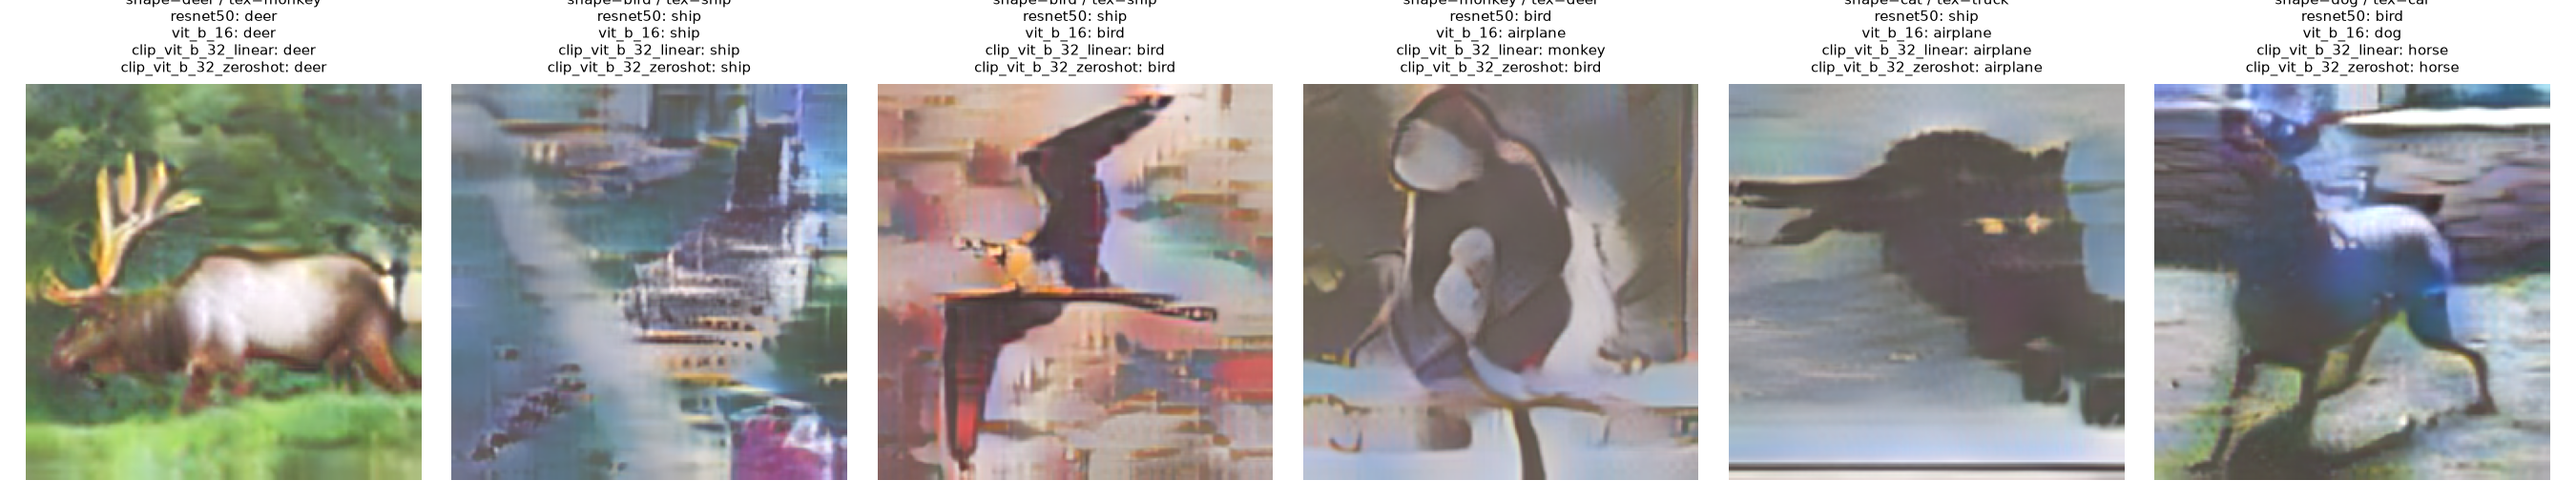
\includegraphics[width=.80\linewidth]{figures/cue_conflict_gallery.png}
\caption{Random samples of accepted cue conflicts. Shape-texture pairs from left to right: deer-monkey, bird-ship, bird-ship, monkey-deer, cat-truck, dog-car.}
\label{fig:cuegallery}
\end{figure}

\begin{table}[t]
    \caption{Cue-conflict decisions over 200 prediction-blind, manually approved images, with 20 images per pair/direction bucket. Bias excludes ``other'' predictions, and coverage exposes that exclusion.}
    \label{tab:cue}\centering\scriptsize
\begin{tabular}{lrrrrr}
\toprule
Model & Shape & Texture & Other & Shape bias & Coverage\\
\midrule
ResNet head & 61 & 45 & 94 & 57.5\% & 53.0\%\\
ViT head & 108 & 19 & 73 & 85.0\% & 63.5\%\\
CLIP head & 126 & 10 & 64 & 92.6\% & 68.0\%\\
CLIP zero-shot & 134 & 10 & 56 & 93.1\% & 72.0\%\\
\bottomrule
\end{tabular}
\end{table}

\begin{figure}[t]
\centering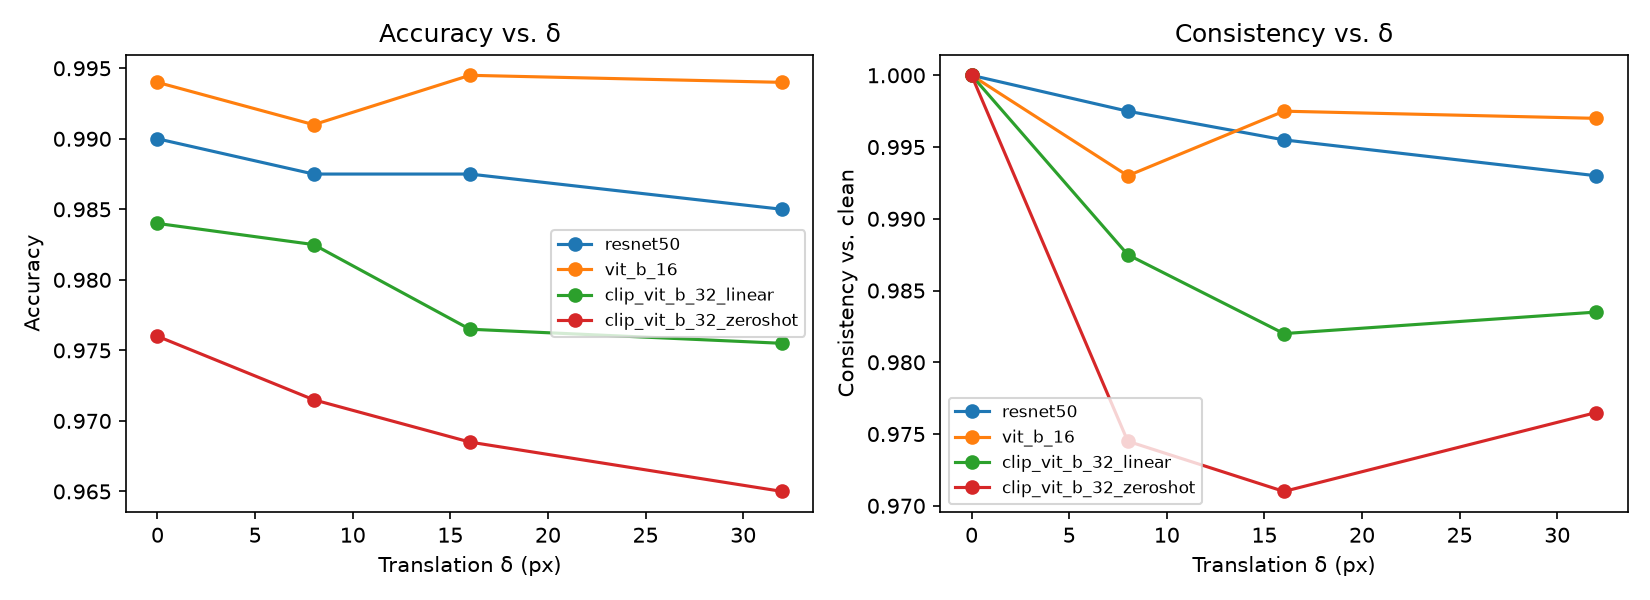
\includegraphics[width=.60\linewidth]{figures/translation_curves.png}
\caption{Accuracy and consistency averaged across translation directions. All models are stable through 32 pixels, although CLIP zero-shot is most position-sensitive and still retains 97.6\% consistency.}
\label{fig:translation}
\end{figure}

Figure~\ref{fig:translation} shows the effect of on each model of increasing the random displacement in the images. Generally, the accuracies remain above $96.5\%$, but the ViT and ResNet models prove to be more resilient than the CLIP models, as their consistency scores remain above $99\%$ while those of the CLIP models drop lower. CNNs are more resistant to positional variance in images, as convolution focuses on local relations. The CLIP zero-shot variant suffers the most, indicating its sensitivity to positional variance when comparing embeddings with the text prompts. Translation is less destructive to model performance than patch shuffling, because translation still preserves the local features and relations between pixels, while patch shuffling completely destroys these relations.

\begin{table}[H]
\caption{Representation stability as the mean cosine similarity between each clean image feature and its transformed counterpart. Higher values mean the paired features remain more similar. The cue-conflict comparison uses the clean content images as its reference.}
\label{tab:reprstability}\centering\scriptsize
\begin{tabular}{@{}lcccc@{}}
\toprule
Backbone & Grayscale & Cue conflict & Translate 32 px up & Patch shuffle\\
\midrule
ResNet-50 & 0.805 & 0.264 & 0.935 & 0.695\\
ViT-B/16 & 0.738 & 0.255 & 0.941 & 0.634\\
CLIP ViT-B/32 & 0.890 & 0.695 & 0.972 & 0.749\\
\bottomrule
\end{tabular}
\end{table}

Table~\ref{tab:reprstability} shows that translation changes the features the least, while cue conflicts change them the most. Figure~\ref{fig:tsne} gives a similar view of the local neighborhoods: translated points mostly remain among clean points of the same class, and grayscale largely retains the clean class groups. Patch shuffling displaces more transformed points, although some class structure remains. The cue-conflict panels show much more mixing between transformed examples and the clean class groups, consistent with the low paired similarity and the high number of ``other'' predictions in Table~\ref{tab:cue}. For CLIP, cue conflict still leaves appreciable cosine similarity even though its transformed points move into different local neighborhoods. Cosine similarity and t-SNE therefore give related but different views of the change. Each panel has its own projection, so we only interpret overlap and mixing within a panel, not distances between panels or backbones.

\FloatBarrier
\section{Unsupervised domain adaptation and domain generalization}
\label{sec:domain}
In Table~\ref{tab:pacs}, we observe a large gap between the shared ERM model's source validation performance and its performance on the target domain. This suggests that training on Photo, Art and Cartoon alone does not make the learned features stable under the change to line drawings. The errors are also uneven across classes. For example, dog and giraffe contribute to many failures, and the animal classes are often confused with one another, while guitar is recognized much more reliably (Appendix Fig.~\ref{fig:pacsconfusion-erm}). Sketches remove much of the color, texture and background information available in the sources, so similar animal outlines may be harder to separate. House also has low accuracy, although its much smaller number of target examples limits how much it contributes to the total error.

\begin{table}[H]
\caption{PACS classification results. The UDA probe measures binary source vs. target domain classification accuracy. $\Delta$ is the target accuracy relative to the shared ERM checkpoint, in percentage points.}
\label{tab:pacs}\centering\scriptsize\setlength{\tabcolsep}{1.5pt}
\resizebox{\linewidth}{!}{%
\begin{tabular}{@{}l*{12}{c}@{}}
\toprule
& \multicolumn{2}{c}{Photo (\%)} & \multicolumn{2}{c}{Art (\%)} & \multicolumn{2}{c}{Cartoon (\%)} & \multicolumn{2}{c}{Mean source (\%)} & \multicolumn{2}{c}{Sketch (\%)} & & \\
\cmidrule(lr){2-3}\cmidrule(lr){4-5}\cmidrule(lr){6-7}\cmidrule(lr){8-9}\cmidrule(lr){10-11}
Method & Accuracy & Macro-F1 & Accuracy & Macro-F1 & Accuracy & Macro-F1 & Accuracy & Macro-F1 & Accuracy & Macro-F1 & $\Delta$ (pp) & UDA probe (\%)\\
\midrule
% \multicolumn{13}{@{}l}{Shared baseline}\\
ERM & 96.7 & 96.1 & 92.4 & 93.1 & 94.9 & 95.3 & 94.7 & 94.8 & 70.1 & 69.2 & 0.0 & 99.7\\
\midrule
% \multicolumn{13}{@{}l}{Unsupervised domain adaptation}\\
DAN & 25.7 & 5.9 & 22.0 & 5.1 & 17.3 & 4.2 & 21.7 & 5.1 & 4.1 & 1.1 & $-66.0$ & 50.0\\
DANN & 18.0 & 17.1 & 15.6 & 14.4 & 16.2 & 14.5 & 16.6 & 15.3 & 19.2 & 13.6 & $-50.9$ & 75.8\\
CDAN & 94.9 & 94.5 & 89.5 & 89.6 & 94.9 & 95.6 & 93.1 & 93.2 & \best{78.1} & \best{76.4} & $+8.0$ & 97.5\\
\midrule
% \multicolumn{13}{@{}l}{Domain generalization}\\
DAN-DG & 25.7 & 5.9 & 22.0 & 5.1 & 17.3 & 4.2 & 21.7 & 5.1 & 4.1 & 1.1 & $-66.0$ & --\\
SAM & 97.9 & 97.5 & 92.7 & 92.6 & 95.7 & 96.3 & \best{95.4} & \best{95.5} & 69.5 & 70.8 & $-0.6$ & --\\
\bottomrule
\end{tabular}}
\end{table}

For UDA, CDAN is the only main adaptation method that improves target recognition while keeping source performance high. Its improvement extends across every class in Fig.~\ref{fig:pacsclass}, which suggests that conditioning alignment on the predicted class helps retain useful distinctions between objects. The domain probe still distinguishes source and target features easily, so complete domain confusion was not needed for this gain. DAN severely underperforms on source classification, and is even worse on target classification, which shows how lower probe accuracy alone should not be taken as success \citep{zhao2019invariant}. Its marginal MMD objective matches the overall feature distributions without checking whether examples from the same class are matched. In our main run, source classification collapses and every target image is predicted as ``person'' (Appendix Fig.~\ref{fig:pacsconfusion-dan}), even though the domain probe is near random chance. This collapse may also be aggravated by a high penalty weight ($\lambda$), as shown in Table~\ref{tab:control} and discussed in the following paragraph. DANN also performs poorly, but its unstable classification and domain losses in Fig.~\ref{fig:pacscurves} make it difficult to separate adversarial alignment from an optimization failure.

The alignment-strength study in Table~\ref{tab:control} shows an abrupt loss of class discrimination as the MMD weight increases, rather than a gradual trade-off between source and target accuracy. With the weaker penalty, DAN can retain the source classes and improve target accuracy, while stronger penalties give the alignment objective more influence over the features used by the classifier. Since MMD matches marginal distributions, reducing it can also pull different classes together, which would explain near random probes and collapsed predictions in the stronger runs. DAN-DG shows the same failure when it aligns pairs of source domains. Thus, for using DAN and DAN-based training schemes, using a weaker $\lambda$ would provide better results for both UDA and DG, although for fairness we keep the preselected main setting for the comparison with other methods. We also tested multiple alternate seeds to see whether the collapse was specific to the original random state, but collapse still appeared in those runs.

For DG, SAM slightly improves mean and worst-source performance and reduces the local sharpness proxy in Table~\ref{tab:dgdiagnostics}, yet its target accuracy remains close to ERM. Its nearly unchanged aggregate metrics also hide a tradeoff observable in Fig.~\ref{fig:pacsclass}, where dog and person worsen while elephant and giraffe improve (Appendix Fig.~\ref{fig:pacsconfusion-sam}). DAN-DG has an even lower sharpness proxy and makes the source domains hard to distinguish, but it loses the ability to classify them and predicts ``person'' for every target image (Appendix Fig.~\ref{fig:pacsconfusion-dan-dg}). A nearly constant classifier can appear stable under this local perturbation while still being useless for recognition. The weaker UDA DAN run ($\lambda = 0.1$) performs better than DAN-DG on the target, suggesting that unlabeled target images may help. However, the methods align different domain pairs, and the same weight can produce different penalties, so target access alone cannot explain the gap.

\begin{figure}[htbp]
\centering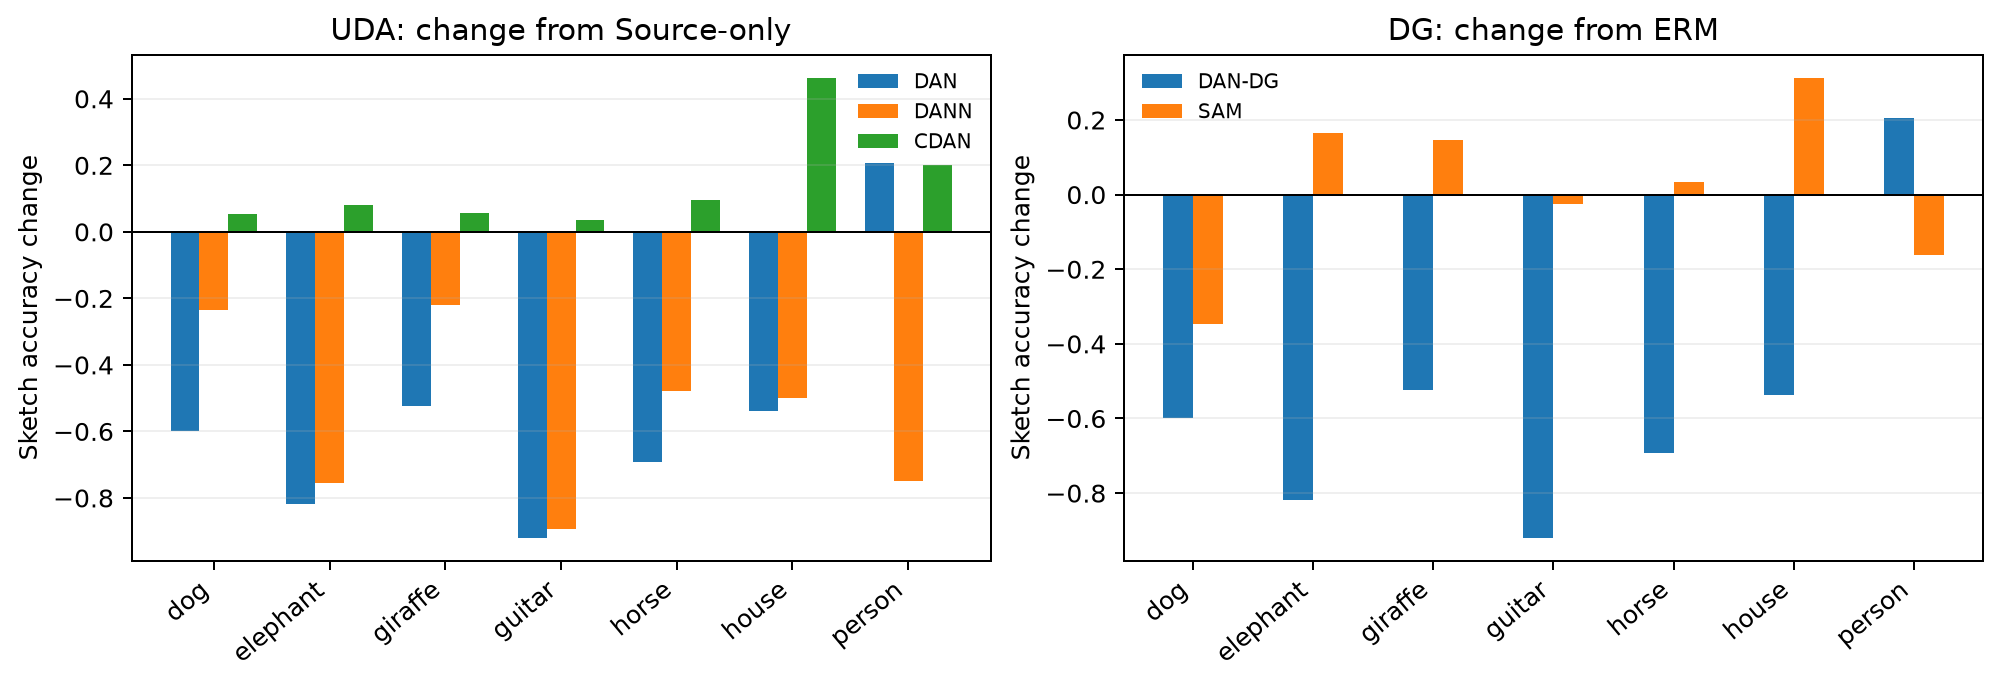
\includegraphics[width=.68\linewidth]{figures/pacs_per_class.png}
\caption{Sketch class-accuracy changes. CDAN improves every class, while marginal alignment causes broad negative transfer. SAM's near-neutral aggregate hides large class trades.}
\label{fig:pacsclass}
\end{figure}

\FloatBarrier
\section{Open-set recognition}
\label{sec:osr}
The Vanilla model classifies most CIFAR-10 test images correctly, but this does not imply that its predictions on unseen classes can be trusted, as can be seen in Table~\ref{tab:scores},which separates ranking unknowns over all thresholds, measured by AUROC, from rejection at the threshold fixed on known validation images. Near unknowns are harder to classify under every score, because they are visually close to a known class, so they can receive the same strong class evidence as CIFAR-10 samples. Far unknowns are overall easier to rank, although the overlap in Fig.~\ref{fig:osrscores} shows that none of the scores separates them completely.

\begin{table}[H]
\caption{A comparison of four unknownness scores using the same frozen Vanilla classifier. AUROC measures how well each score ranks known test images against near, far, or all unknowns. The acceptance and rejection rates use a separate threshold for each score, set from known validation images to accept approximately 95\% of them.}
\label{tab:scores}\centering\scriptsize\setlength{\tabcolsep}{4pt}
\begin{tabular}{@{}l*{6}{c}@{}}
\toprule
& \multicolumn{3}{c}{AUROC (\%)} & \multicolumn{1}{c}{Known test (\%)} & \multicolumn{2}{c}{Unknown rejected (\%)}\\
\cmidrule(lr){2-4}\cmidrule(lr){5-5}\cmidrule(l){6-7}
Score & Near & Far & All & Accepted & Near & Far\\
\midrule
MSP & \best{81.1} & 89.5 & 85.3 & 95.0 & 28.4 & 43.6\\
MLS & 79.3 & 89.4 & 84.4 & 95.4 & 30.6 & 55.0\\
Energy & 79.3 & 89.5 & 84.4 & \best{95.6} & 30.5 & \best{56.3}\\
Mahalanobis & 79.3 & \best{91.8} & \best{85.5} & 95.2 & 27.0 & 50.6\\
\bottomrule
\end{tabular}
\end{table}

MSP \citep{hendrycks2017baseline} uses the largest normalized class probability and gives the best near-unknown ranking among the four vanilla scores. However, normalization can still hide the absolute size of the logits, because a sample may have a dominant class probability even when all class logits are weak. MLS \citep{vaze2022osr} instead uses the largest logit directly. Energy \citep{liu2020energy} combines evidence from all logits, but its near-identical behavior to MLS here suggests that one class response dominates the sum value.
Mahalanobis distance \citep{lee2018mahalanobis} measures distance to the nearest known class feature cluster, and ranks far unknowns best overall, yet rejects fewer of them than MLS and Energy at the validation-calibrated threshold. Its feature distances are therefore useful for ordering many far examples, but that advantage does not carry over to this particular threshold.

\begin{table}[H]
\caption{A comparison of the three trained models using the same maximum-logit score (MLS), along with PROSER's placeholder-based Delta-P score. Accuracy measures classification among the ten CIFAR-10 classes, while AUROC measures known vs. unknown ranking. Acceptance and rejection use a threshold calibrated separately for each model and score on known validation images.}
\label{tab:osrmodels}\centering\scriptsize\setlength{\tabcolsep}{3pt}
\begin{tabular}{@{}ll*{7}{c}@{}}
\toprule
& & \multicolumn{2}{c}{Known test (\%)} & \multicolumn{3}{c}{AUROC (\%)} & \multicolumn{2}{c}{Unknown rejected (\%)}\\
\cmidrule(lr){3-4}\cmidrule(lr){5-7}\cmidrule(l){8-9}
Model & Score & Accuracy & Accepted & Near & Far & All & Near & Far\\
\midrule
Vanilla & MLS & 94.7 & 95.4 & 79.3 & 89.4 & 84.4 & 30.6 & 55.0\\
GCSC & MLS & \best{95.2} & 95.2 & 80.4 & \best{92.1} & \best{86.2} & \best{34.3} & \best{63.6}\\
PROSER & MLS & 94.5 & 95.5 & \best{81.2} & 87.1 & 84.2 & 31.0 & 45.5\\
PROSER & Delta-P & 94.5 & \best{95.7} & 79.7 & 88.1 & 83.9 & 28.6 & 44.8\\
\bottomrule
\end{tabular}
\end{table}

Under the common MLS score in Table~\ref{tab:osrmodels}, GCSC improves both known-class accuracy and unknown rejection, with a clearer gain on far unknowns. RandAugment exposes the classifier to stronger changes of known images during training, which may make its learned class evidence less dependent on incidental appearance, allowing more unfamiliar images to receive lower known-class logits. While this is a useful gain in this experiment, known-class accuracy alone does not determine how safely a classifier rejects unknowns.

PROSER behaves differently. Its MLS score ranks near unknowns slightly better than vanilla, which is consistent with mixed features providing training examples between known classes. At the fixed acceptance rate, however, near rejection changes little and far rejection worsens. This is because the mixed features only cover regions formed from the available known classes, but they do not necessarily resemble far unknowns such as household objects. PROSER also loses some closed set accuracy, so the extra dummy-class objective does not improve both recognition along with rejection here. Its own placeholder Delta-P score slightly improves far-unknown AUROC over PROSER's MLS score, but lowers overall AUROC and both rejection rates. A strong dummy response therefore does not give a better rejection rule at this operating point for these held-out classes.

\begin{figure}[H]
\centering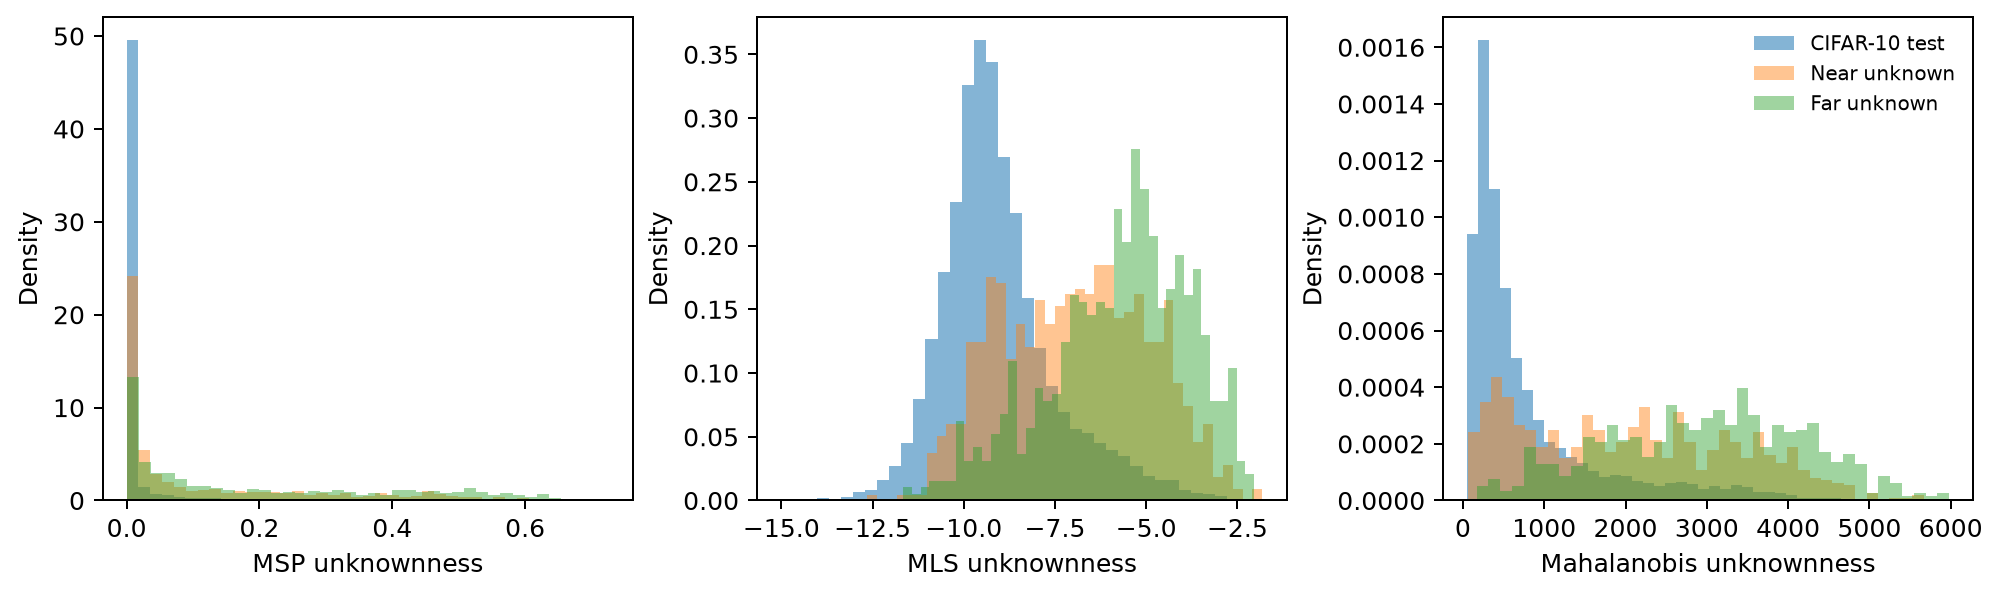
\includegraphics[width=.65\linewidth]{figures/osr_scores.png}
\caption{Unknownness scores from the frozen Vanilla classifier for known CIFAR-10 test images and the two CIFAR-100 unknown class groups. Larger scores indicate greater unknownness. Near unknowns overlap known examples more strongly than far unknowns, which limits rejection when the threshold must still accept most known images.}
\label{fig:osrscores}
\end{figure}

The class-level results in Appendix Fig.~\ref{fig:unknownacceptance} show why the aggregate near/far difference should not be treated as a clean semantic boundary. For instance, wolf and pickup truck are among the most frequently accepted near classes, usually mapped to cat and automobile, respectively.
Their visual similarity to known classes makes these failures understandable. Among the far classes, wardrobe is accepted most often and is frequently assigned to truck, showing that a nominally far class can still trigger strong known-class evidence. At a fixed Vanilla MLS threshold, every example in Table~\ref{tab:failures} has an unknownness score below the cutoff and is therefore accepted. Bus to truck and fox to dog are plausible confusions, but mismatches like clock to airplane, keyboard to frog and mushroom to bird show that high known-class logits can also arise without an obvious semantic match. The threshold was calibrated to retain known images, so these failures were not corrected using the unknown labels after inspection as to keep the analysis purely OSR-related.

\begin{table}[H]
\caption{The three most confidently accepted near and far unknowns under the Vanilla MLS score. Each score falls below the known validation threshold $\tau=-5.745$, so the model accepts the image as the predicted CIFAR-10 class. The assessment distinguishes visually plausible matches from surprising ones.}
\label{tab:failures}\centering\scriptsize
\begin{tabular}{llllr}
\toprule
Group & Unknown & Predicted known & Assessment & $u_{\mathrm{MLS}}$\\
\midrule
Near & bus & truck & plausible & $-12.641$\\
Near & fox & dog & plausible & $-11.664$\\
Near & bus & truck & plausible & $-11.297$\\
Far & clock & airplane & surprising & $-11.664$\\
Far & keyboard & frog & surprising & $-11.523$\\
Far & mushroom & bird & surprising & $-11.414$\\
\bottomrule
\end{tabular}
\end{table}

\FloatBarrier
\section{Cross-task synthesis}
The above sections examine different ways in which a classifier can fail outside its clean training setting. However, changing the visual cues of an image, shifting to a new image domain or presenting a new class unknown at training are completely different scenarios individually. Piecing together what we learn from these findings, we now discuss which information a representation must retain to distinguish objects, which variation it can ignore, and when a prediction should be skipped.

\paragraph{What to retain?}\mbox{}\par
The visual interventions in Section~\ref{sec:visual} suggest that a useful representation should preserve the relations between object parts while tolerating changes in position. Translation keeps the image content and local arrangement intact, which explains why both predictions and features remain stable. Patch shuffling retains the pixels but breaks their global arrangement, and cue conflicts put shape and texture evidence in opposition, thus patch shuffling lowers accuracy while cue conflicts often produce predictions outside the two intended classes. In the PACS UDA scenario of Section~\ref{sec:domain}, the target Sketch images lose much of the color and texture seen in the source domains, while similar animal outlines become harder to distinguish. The relatively small effect of grayscale compared to the other visual interventions in Section~\ref{sec:visual} suggests against attributing the domain adaptation gap to missing color alone. Changes in texture detail and background may also contribute, but these experiments use different datasets and models, so this comparison cannot isolate a cause.

\paragraph{What to suppress?}\mbox{}\par
The UDA and DG experiments in Section~\ref{sec:domain} suggest that domain-specific information may be worth suppressing only while the classes remain distinguishable, considering CDAN improves target recognition across classes even though its features remain easy to separate by domain, suggesting that complete domain confusion is unnecessary for useful transfer. DAN and DAN-DG show the opposite failure, as their probes approach random probability while source classification collapses, and most target examples receive the same label. Reducing the alignment weight lets the models retain source classes better while improving target accuracy (which is consistent with excessive marginal alignment pulling different classes together), although performance across source and domain classes are largely comparable to the baseline. SAM also lowers the measured sharpness without a comparable target gain, so a flatter source loss does not by itself address the visual shift. The weaker target-aware DAN run ($\lambda=0.1$) does better than DAN-DG, which suggests that unlabeled target images can help choose what to align. Since the two methods align different domain pairs and apply different effective penalties, this comparison can not comprehensively isolate the effect of target access.

\paragraph{What to reject?}\mbox{}\par
Open-set recognition in Section~\ref{sec:osr} gives us the decision of whether an image belongs to any class the model has learned. GCSC improves known-class classification and unknown rejection together thanks to RandAugment producing class evidence that depends less on incidental appearance, and thus rejects unfamiliar inputs. However, PROSER does not follow the same pattern, as its placeholder objective gives a fair improvement in ranking near unknowns, yet this very improvement does not carry over to rejection at the validation-calibrated threshold, since the mixed features it trains on only mixes between known classes, so they can not resemble actual unknown image classes.
Thus, retaining class evidence is useful for recognition, but the decision to remove it needs its own evaluation rather than being inferred from closed-set accuracy or ranking metrics like AUROC.

\FloatBarrier
\section{Conclusion and limitations}
Across the visual interventions, the models are more stable to changes in color and position than to changes that disrupt the arrangement of object parts or put shape and texture in conflict. This suggests that useful invariance depends on which information is removed, since ignoring a shift in position can preserve recognition while ignoring distinctions between classes cannot. The domain experiments show the latter failure clearly. DAN and DAN-DG become difficult to distinguish by domain, but their class predictions collapse, including in alternate-seed runs. CDAN improves target recognition while its features remain distinguishable by domain. Thus, our results do not support making features domain-indistinguishable as a goal by itself, and class performance has to be checked alongside alignment.

Access to unlabeled target images can help, as CDAN improves on the source-only ERM baseline, while SAM improves source performance and reduces measured sharpness without a similar target gain. However, this comparison also changes the training objective, so we cannot attribute CDAN's gain to target access alone. In OSR, stronger known class training improves recognition and rejection together for GCSC, whereas PROSER's small improvement in ranking near unknowns does not produce a similar improvement in rejection at the chosen threshold. We therefore need to check class accuracy alongside domain separability, and rejection at a calibrated threshold alongside AUROC.

These conclusions are limited by the scope of the experiments. Most main results use one split and one seed, so small differences, including the apparent benefit of color swapping for ViT, may be the result of noise,and may not persist over multiple seeds. Additionally, there is no consistency in the baselines and methodology across all the experiments, as the cue-conflict evaluation uses 200 human-approved images from five class pairs using the STL-10 dataset, PACS uses Sketch as its only target domain, and the open-set study uses an architecture modified for CIFAR and fixed groups of unknown classes. Our rejection results also describe one validation-calibrated operating point. Repeating the experiments across splits and seeds with uncertainty intervals, testing more cue-conflict pairs and target domains, and evaluating rejection across a wider range of unknown classes and thresholds would show which trends are stable. The optimization failures of DAN and DANN also warrant a more controlled study of alignment strength and adversarial-training stability before we are able to confidently draw broader conclusions about these methods.

\clearpage
\bibliographystyle{plainnat}
{\small\bibliography{references}}

\appendix
\numberwithin{figure}{section}
\numberwithin{table}{section}
\section{Embedding visualizations}
\begin{figure}[h]
\centering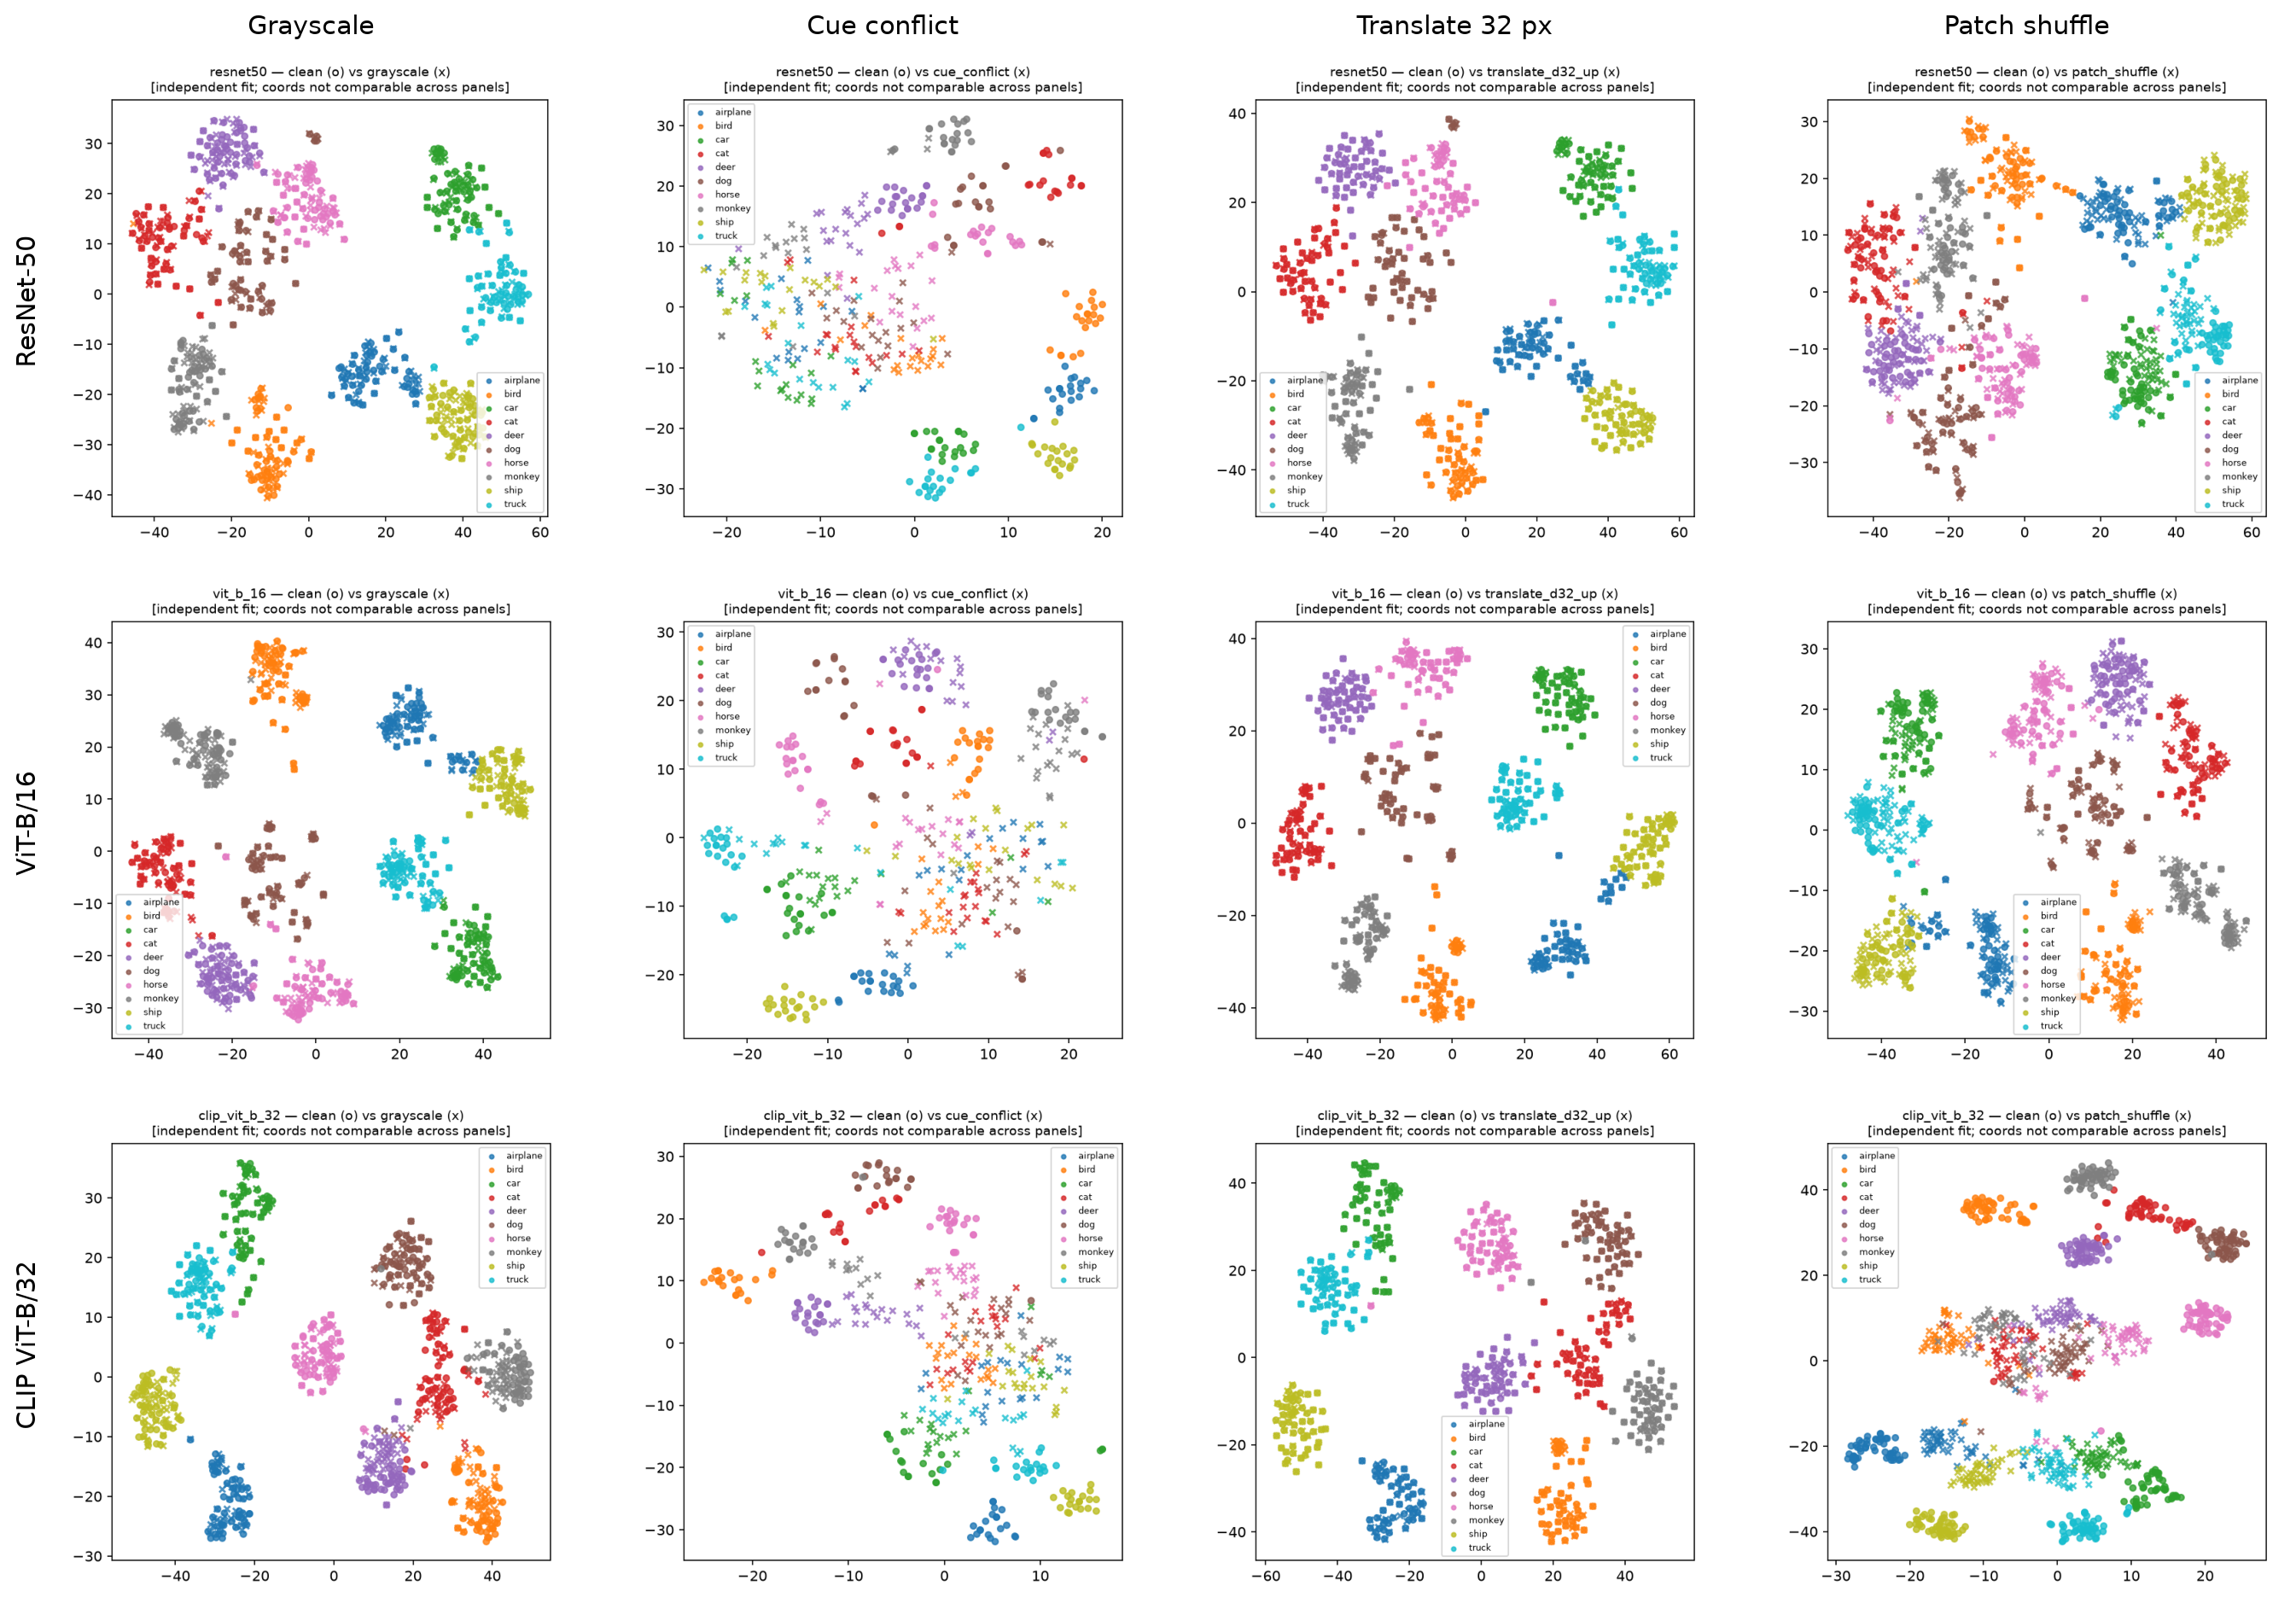
\includegraphics[width=.90\linewidth]{figures/task1_tsne_grid.png}
\caption{Each panel jointly projects clean and transformed features using t-SNE \citep{vandermaaten2008tsne} with cosine distance, perplexity 30 and a seed derived from 6304, with backbones in rows and interventions in columns. Color denotes content class and marker denotes condition. Translation mostly overlaps clean clusters, while cue conflicts mix classes. Coordinates are not compared across panels.}
\label{fig:tsne}
\end{figure}

\section{Open-set supplementary diagnostics}

% \begin{figure}[h]
% \centering\includegraphics[width=.82\linewidth]{figures/multiseed_accuracy.png}
% \caption{Fixed-split training-seed validation. Dashed lines are the preregistered collapse thresholds. DAN is bimodal, DAN-DG collapses for all seeds, and DANN remains poor and numerically unstable.}
% \end{figure}

\begin{figure}[h]
\centering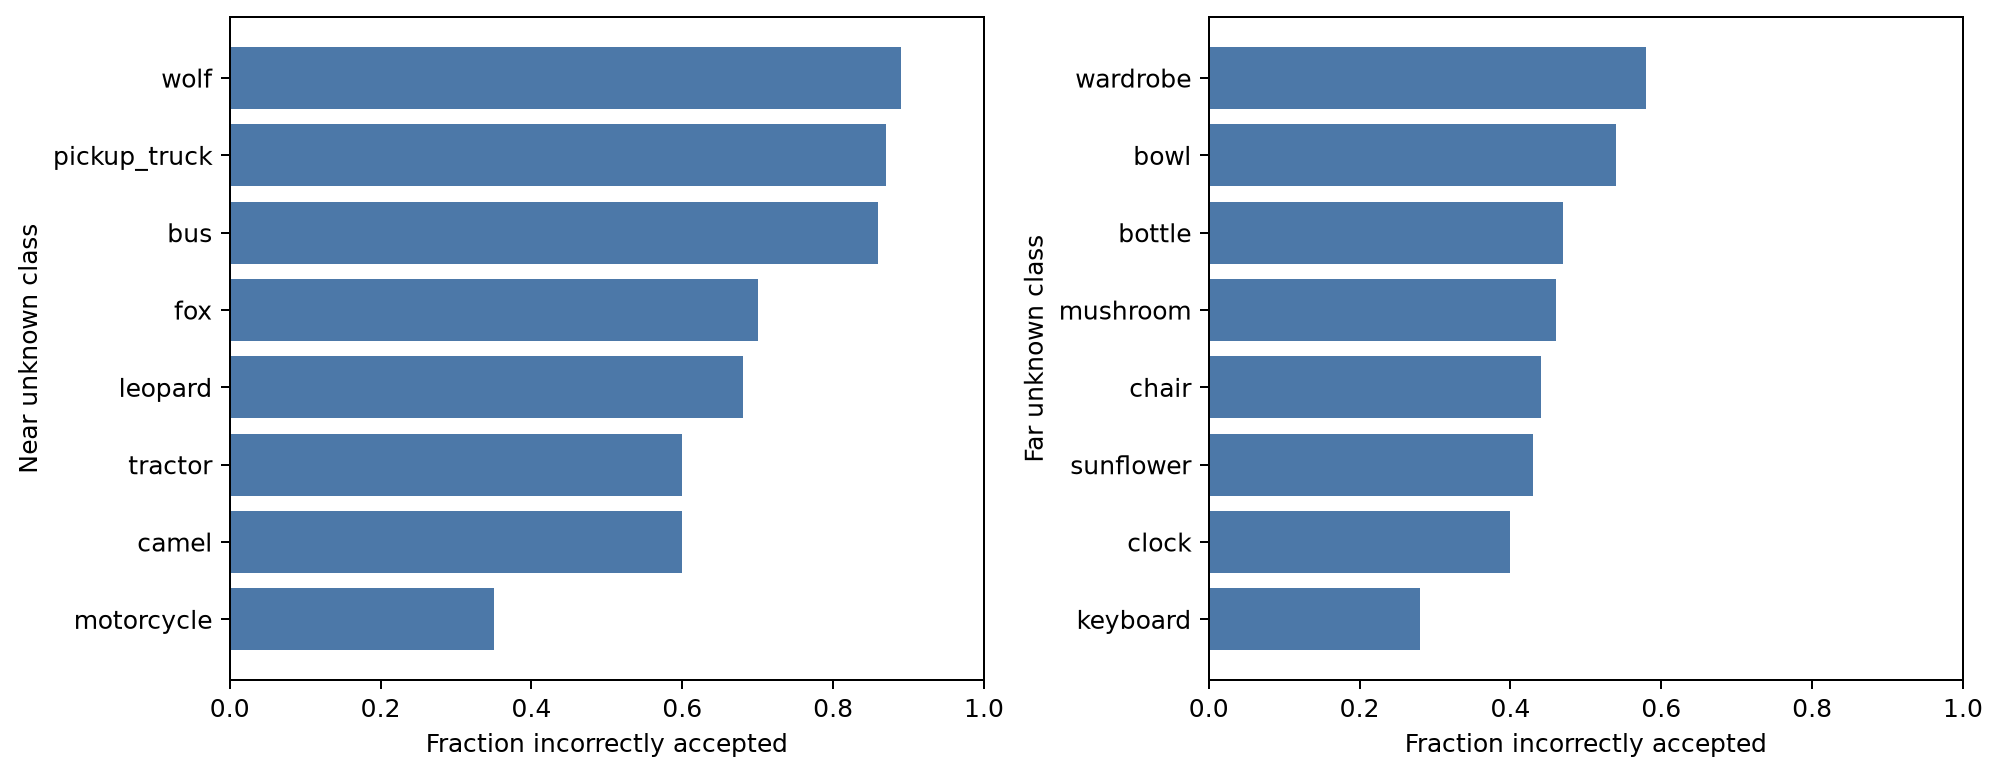
\includegraphics[width=.9\linewidth]{figures/unknown_acceptance.png}
\caption{Class-level Vanilla-MLS acceptance. Near semantic neighbors are accepted most often, but some far classes also map confidently into known labels.}
\label{fig:unknownacceptance}
\end{figure}

\section{PACS supplementary diagnostics}
\begin{figure}[h]
\centering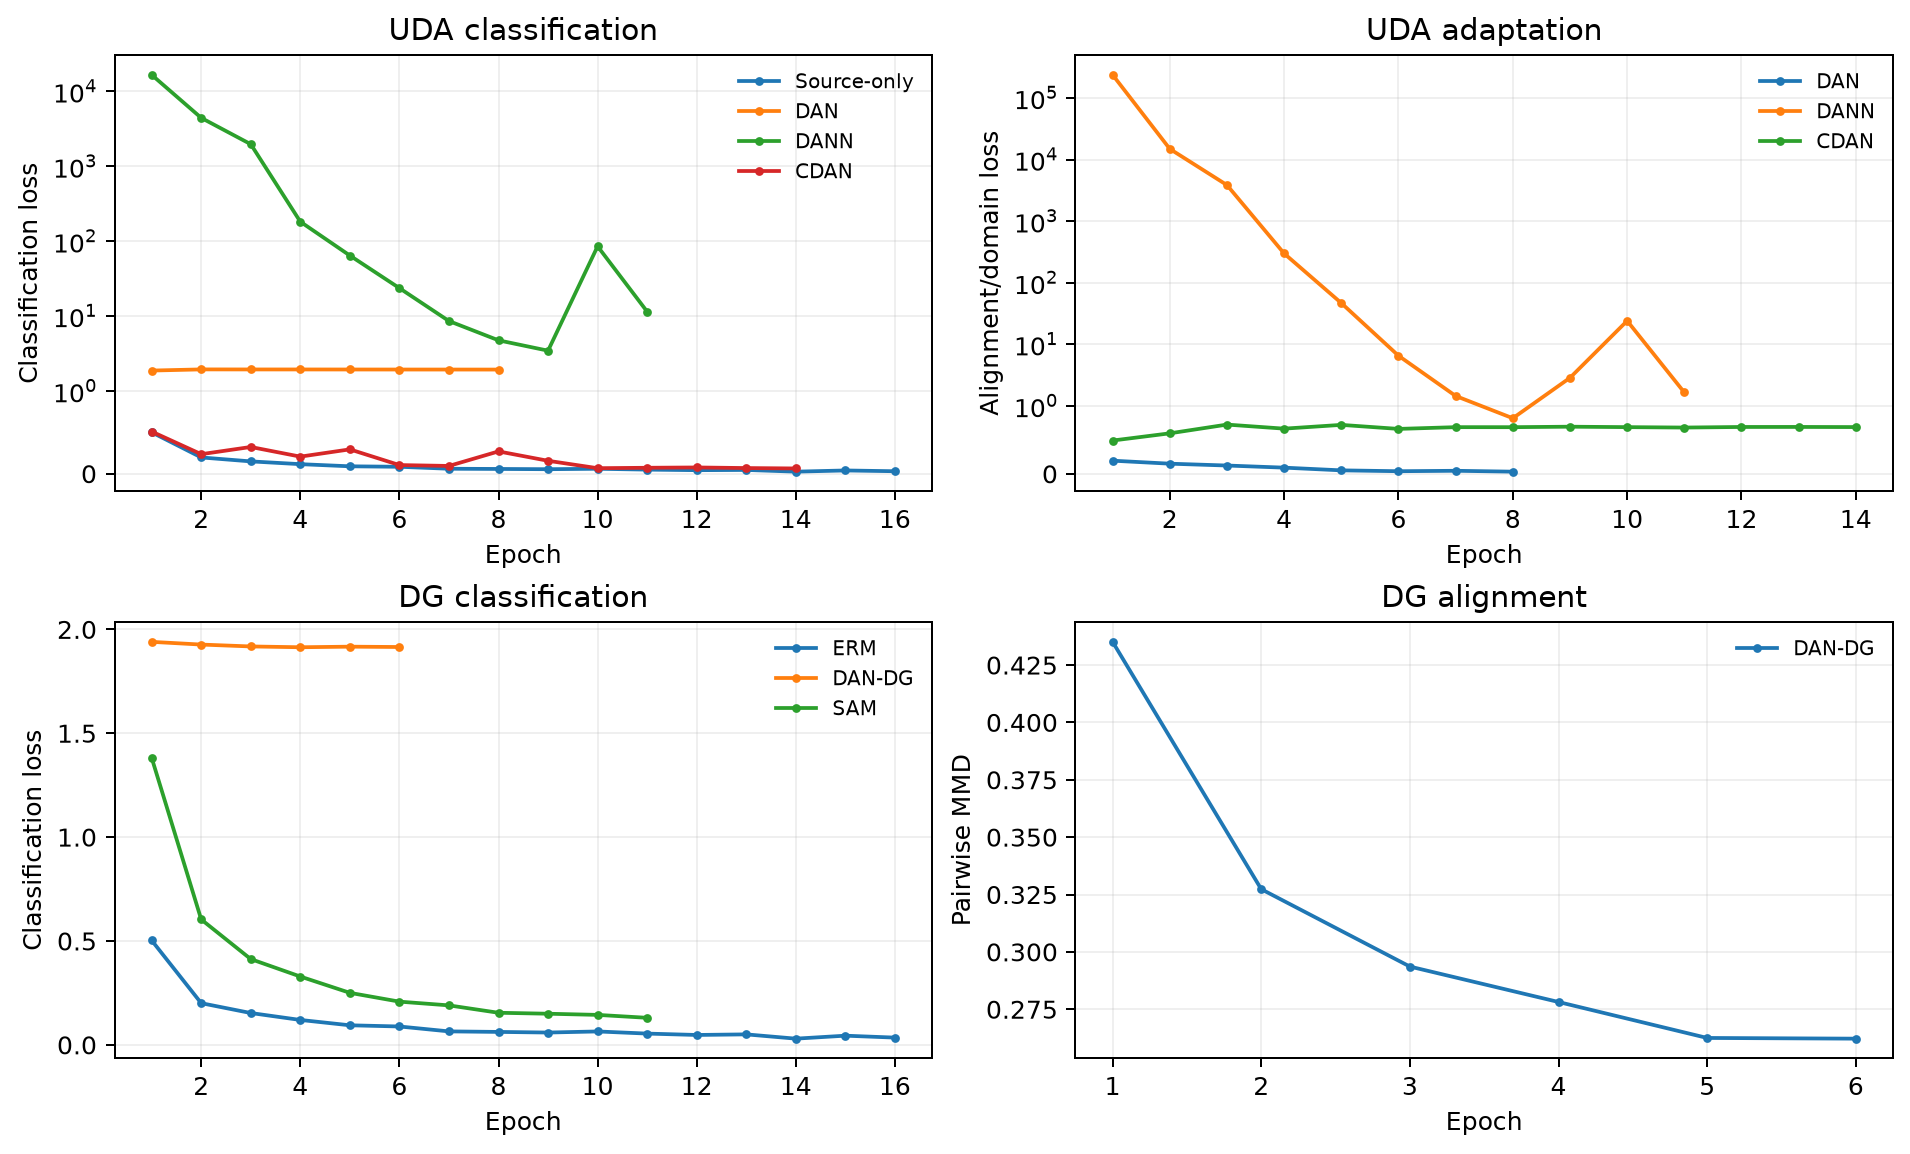
\includegraphics[width=.80\linewidth]{figures/pacs_training_curves.png}
\caption{PACS training curves. Symmetric-log UDA axes expose DANN's exploding losses. DAN and DAN-DG remain near chance-level classification loss, whereas ERM, CDAN, and SAM optimize normally.}
\label{fig:pacscurves}
\end{figure}

\begin{table}[H]
\caption{DG-only diagnostics. The source probe classifies Photo, Art Painting, and Cartoon from frozen features (chance accuracy 33.3\%). Sharpness is the increase in cross-entropy loss after one radius-0.05 parameter perturbation.}
\label{tab:dgdiagnostics}\centering\scriptsize
\begin{tabular}{@{}lcccc@{}}
\toprule
& \multicolumn{2}{c}{Worst source (\%)} & & \\
\cmidrule(lr){2-3}
Method & Accuracy & Macro-F1 & Source probe (\%) & Sharpness (nats)\\
\midrule
ERM & 92.4 & 93.1 & 85.0 & 0.383\\
DAN-DG & 17.3 & 4.2 & 30.2 & 0.032\\
SAM & \best{92.7} & \best{92.6} & 87.4 & 0.133\\
\bottomrule
\end{tabular}
\end{table}

\begin{table}[H]
\caption{Alignment-strength studies. Domain-probe chance accuracy is 50\% for DAN and 33.3\% for DAN-DG.}
\label{tab:control}\centering\scriptsize
\begin{tabular}{@{}llccccc@{}}
\toprule
& & \multicolumn{2}{c}{Mean source (\%)} & & \multicolumn{2}{c}{Sketch (\%)}\\
\cmidrule(lr){3-4}\cmidrule(l){6-7}
Study & $\lambda$ & Accuracy & Macro-F1 & Domain probe (\%) & Accuracy & Macro-F1\\
\midrule
\multirow{3}{*}{DAN} & .1 & 95.3 & 95.1 & 92.7 & 74.6 & 71.1\\
& 1 & 21.7 & 5.1 & 50.0 & 4.1 & 1.1\\
& 10 & 21.7 & 5.1 & 56.2 & 4.1 & 1.1\\
\midrule
\multirow{3}{*}{DAN-DG} & .1 & 95.1 & 95.2 & 76.1 & 67.5 & 69.3\\
& 1 & 21.7 & 5.1 & 30.2 & 4.1 & 1.1\\
& 10 & 21.7 & 5.1 & 33.2 & 4.1 & 1.1\\
\bottomrule
\end{tabular}
\end{table}

\FloatBarrier
\section{PACS target confusion matrices}
\begin{figure}[H]
\centering
\begin{subfigure}{.48\linewidth}
\centering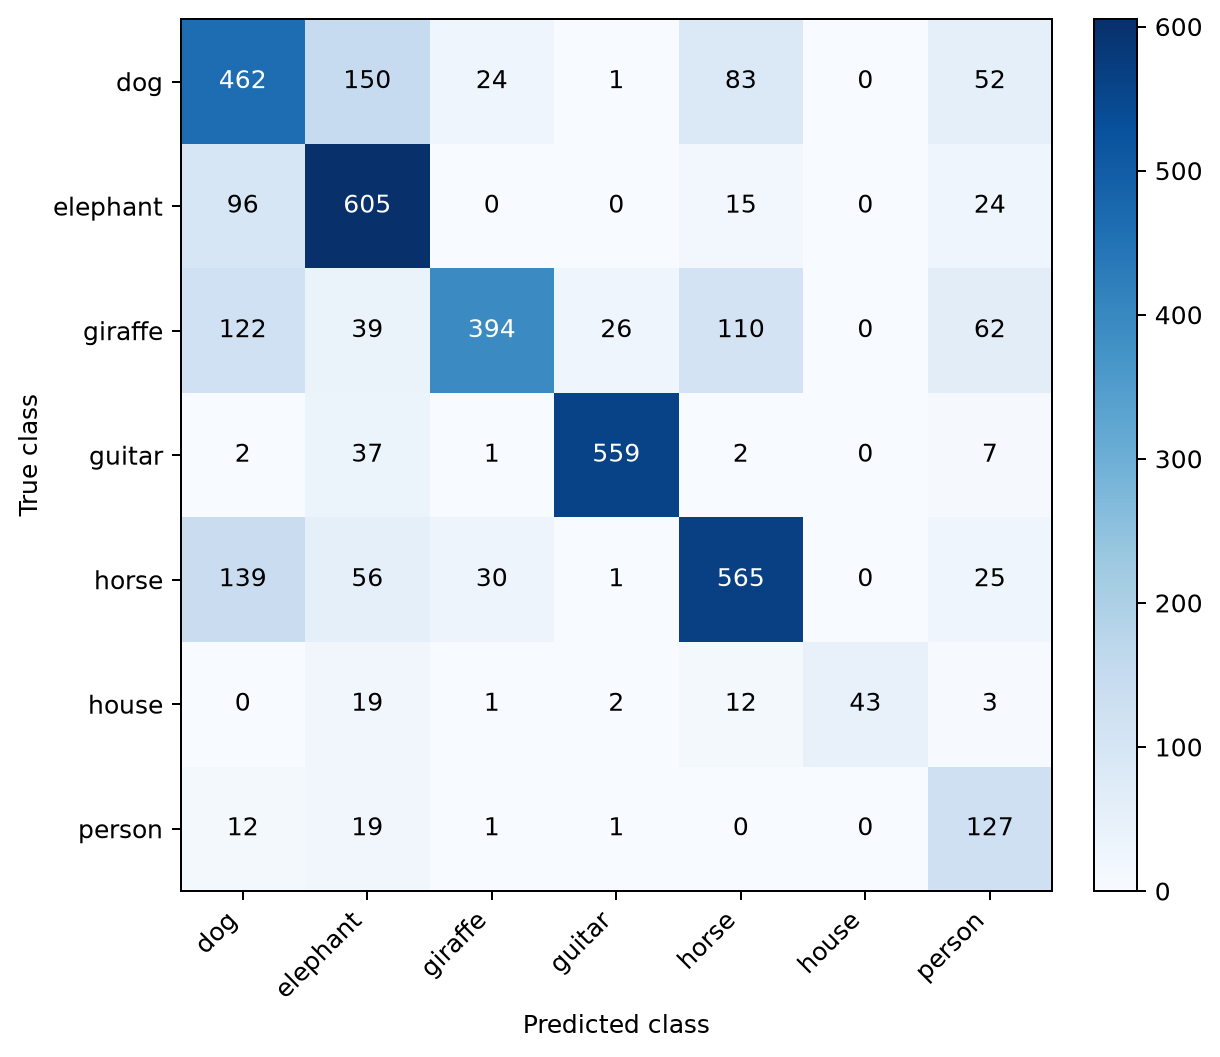
\includegraphics[width=\linewidth]{figures/pacs_confusion_erm.png}
\caption{Shared ERM baseline}\label{fig:pacsconfusion-erm}
\end{subfigure}\hfill
\begin{subfigure}{.48\linewidth}
\centering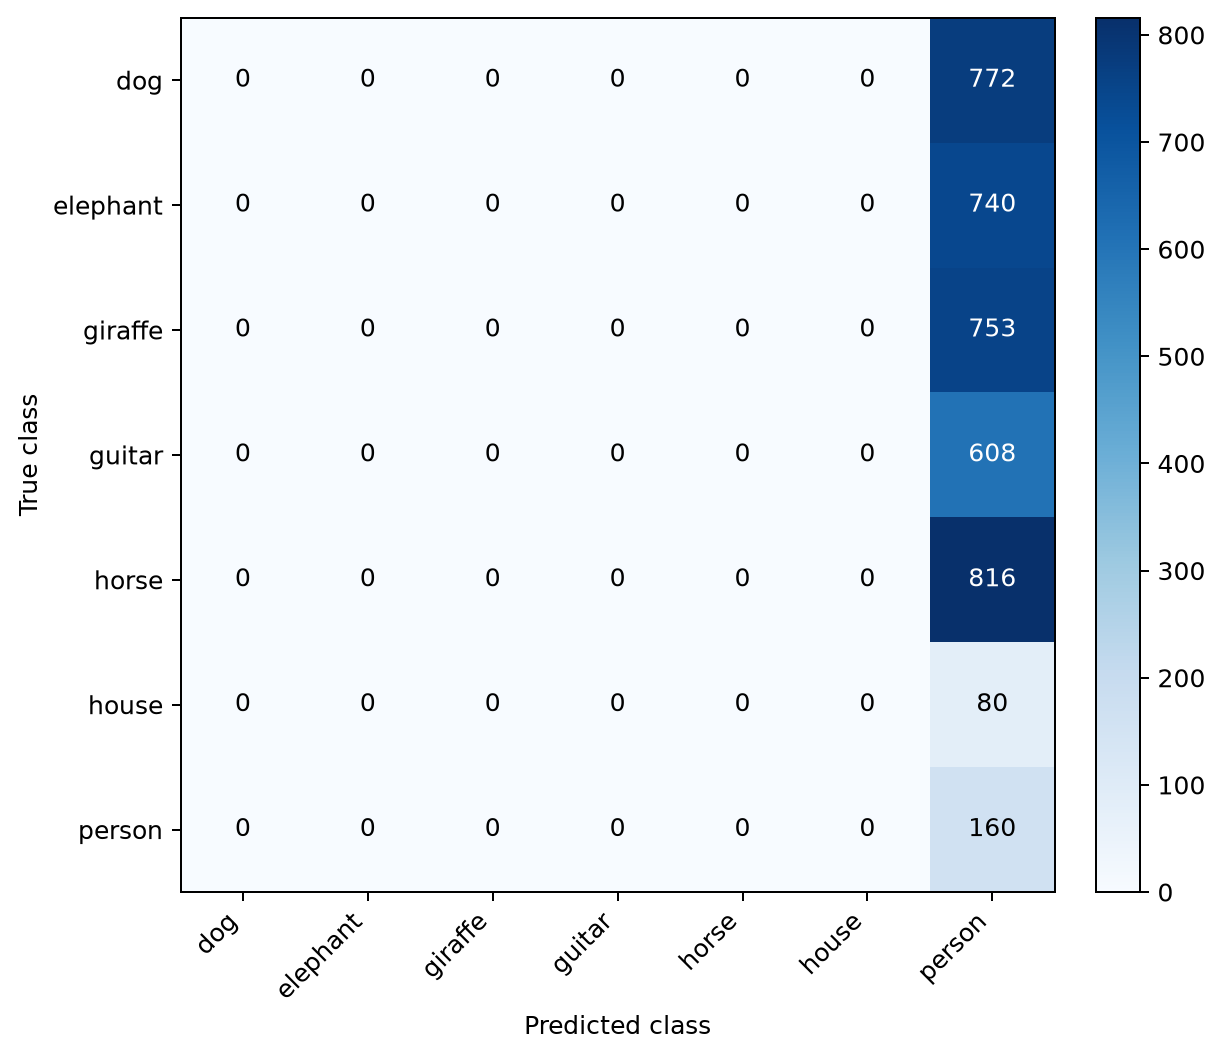
\includegraphics[width=\linewidth]{figures/pacs_confusion_dan.png}
\caption{DAN}\label{fig:pacsconfusion-dan}
\end{subfigure}

\begin{subfigure}{.48\linewidth}
\centering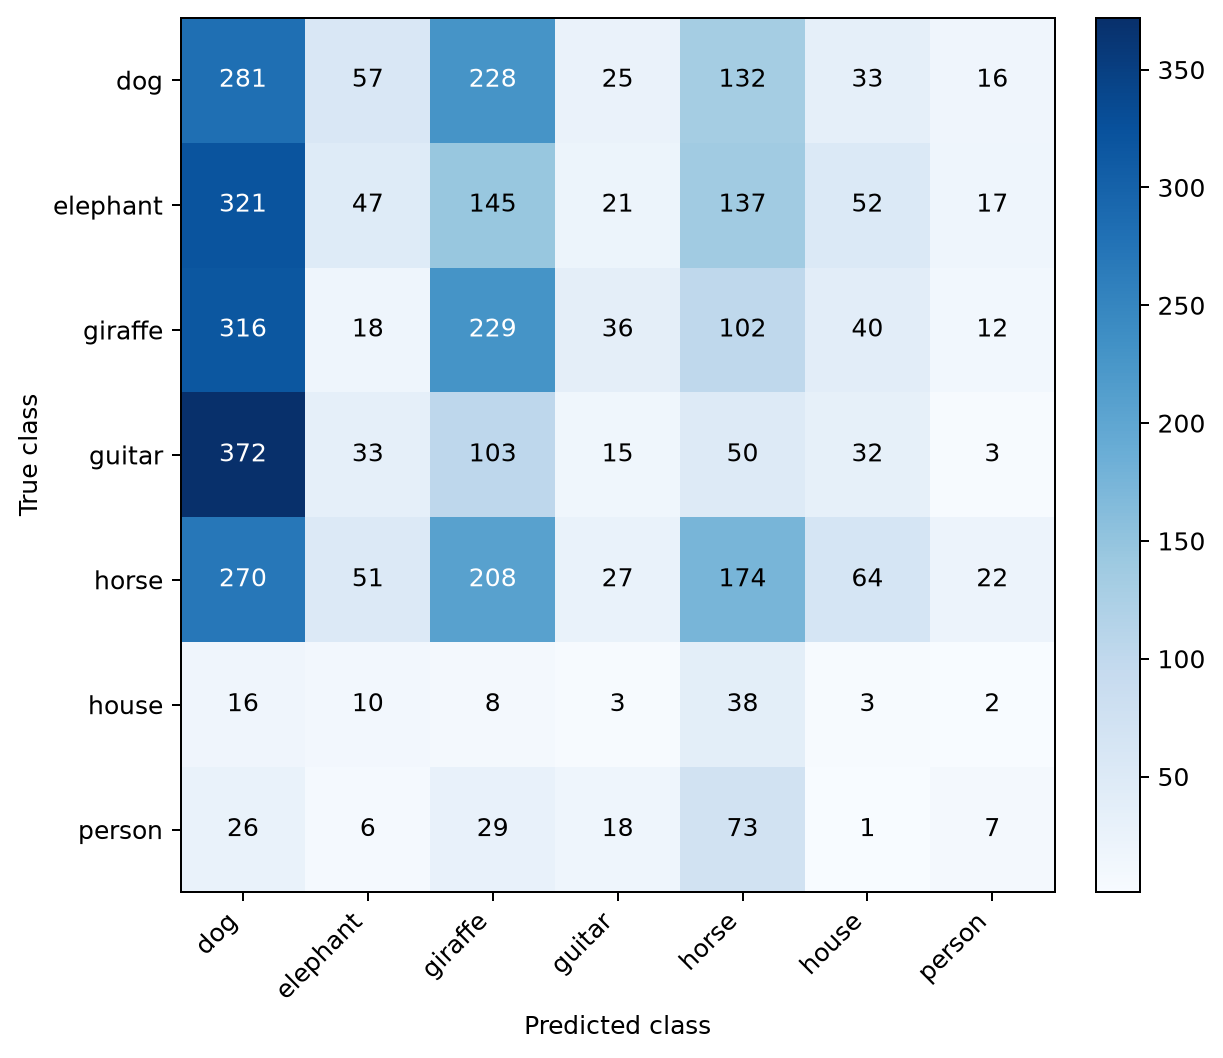
\includegraphics[width=\linewidth]{figures/pacs_confusion_dann.png}
\caption{DANN}\label{fig:pacsconfusion-dann}
\end{subfigure}\hfill
\begin{subfigure}{.48\linewidth}
\centering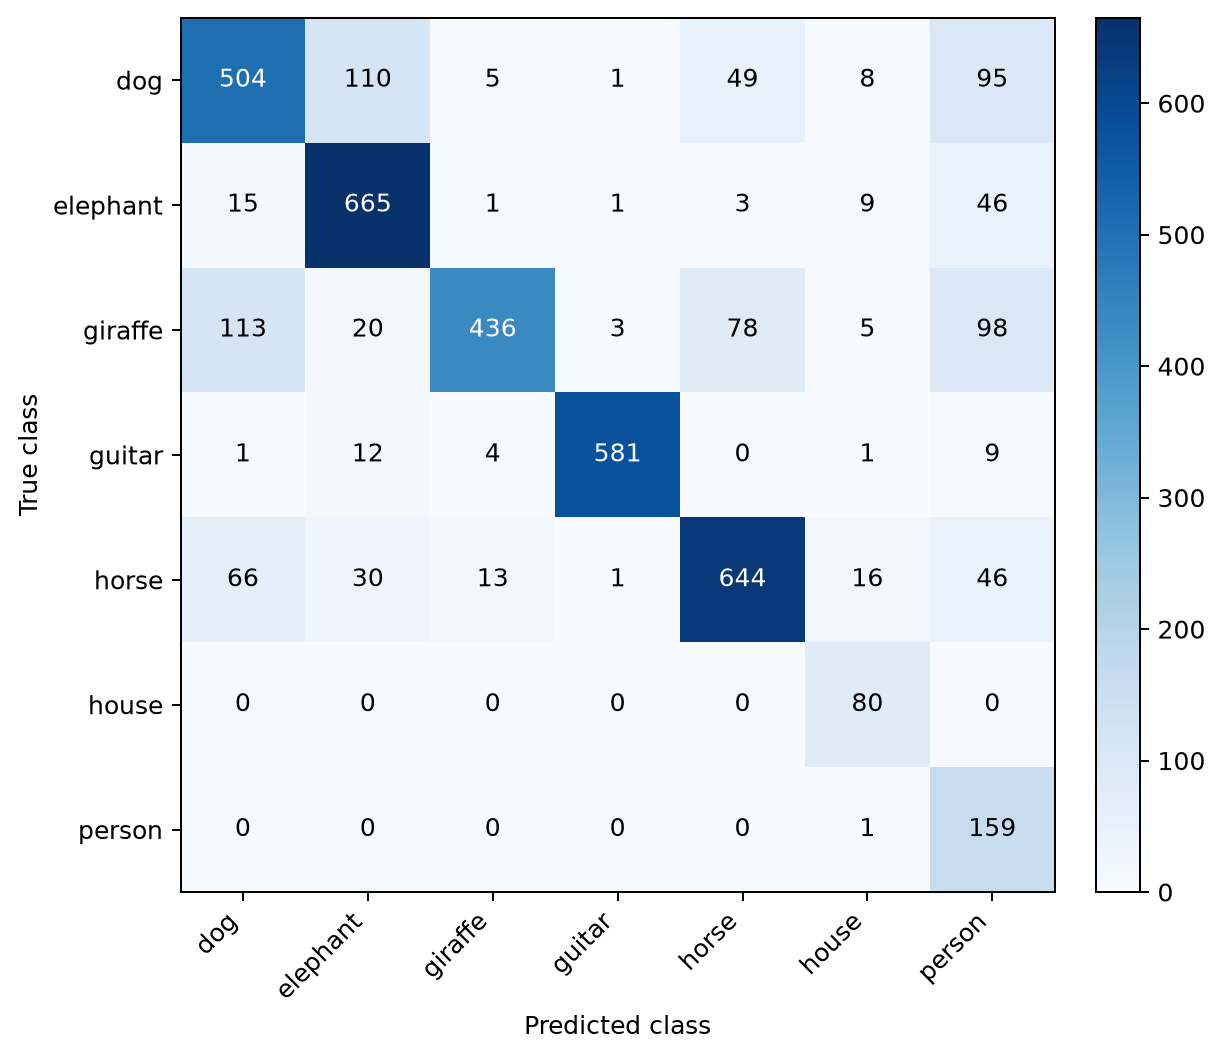
\includegraphics[width=\linewidth]{figures/pacs_confusion_cdan.png}
\caption{CDAN}\label{fig:pacsconfusion-cdan}
\end{subfigure}
\caption{Target-domain confusion matrices for the shared ERM baseline and UDA methods. Rows show true classes, columns show predicted classes, and entries are image counts.}
\label{fig:pacsconfusion-uda}
\end{figure}

\begin{figure}[H]
\centering
\begin{subfigure}{.48\linewidth}
\centering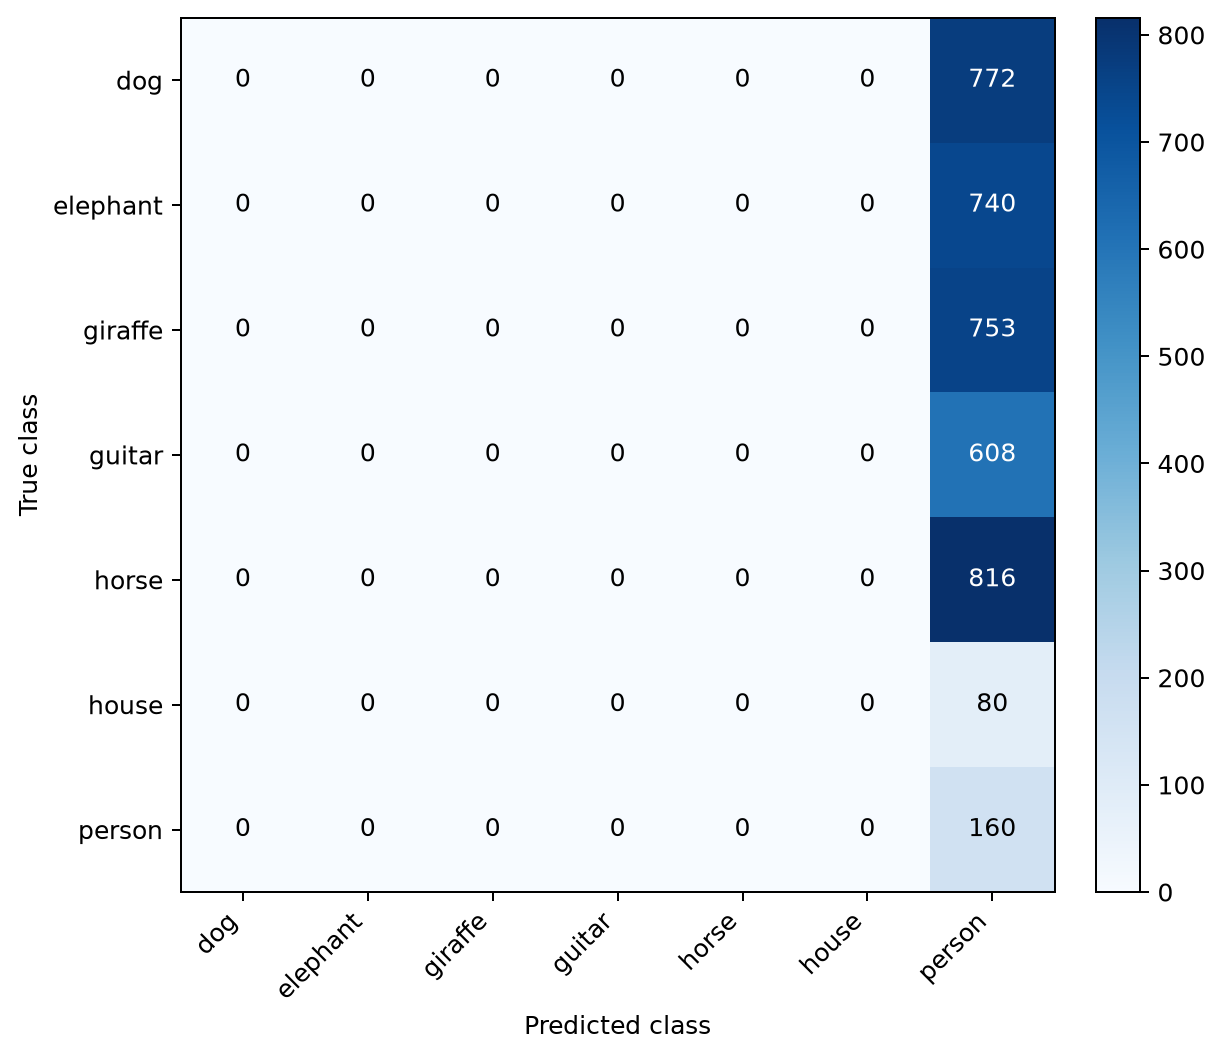
\includegraphics[width=\linewidth]{figures/pacs_confusion_dan_dg.png}
\caption{DAN-DG}\label{fig:pacsconfusion-dan-dg}
\end{subfigure}\hfill
\begin{subfigure}{.48\linewidth}
\centering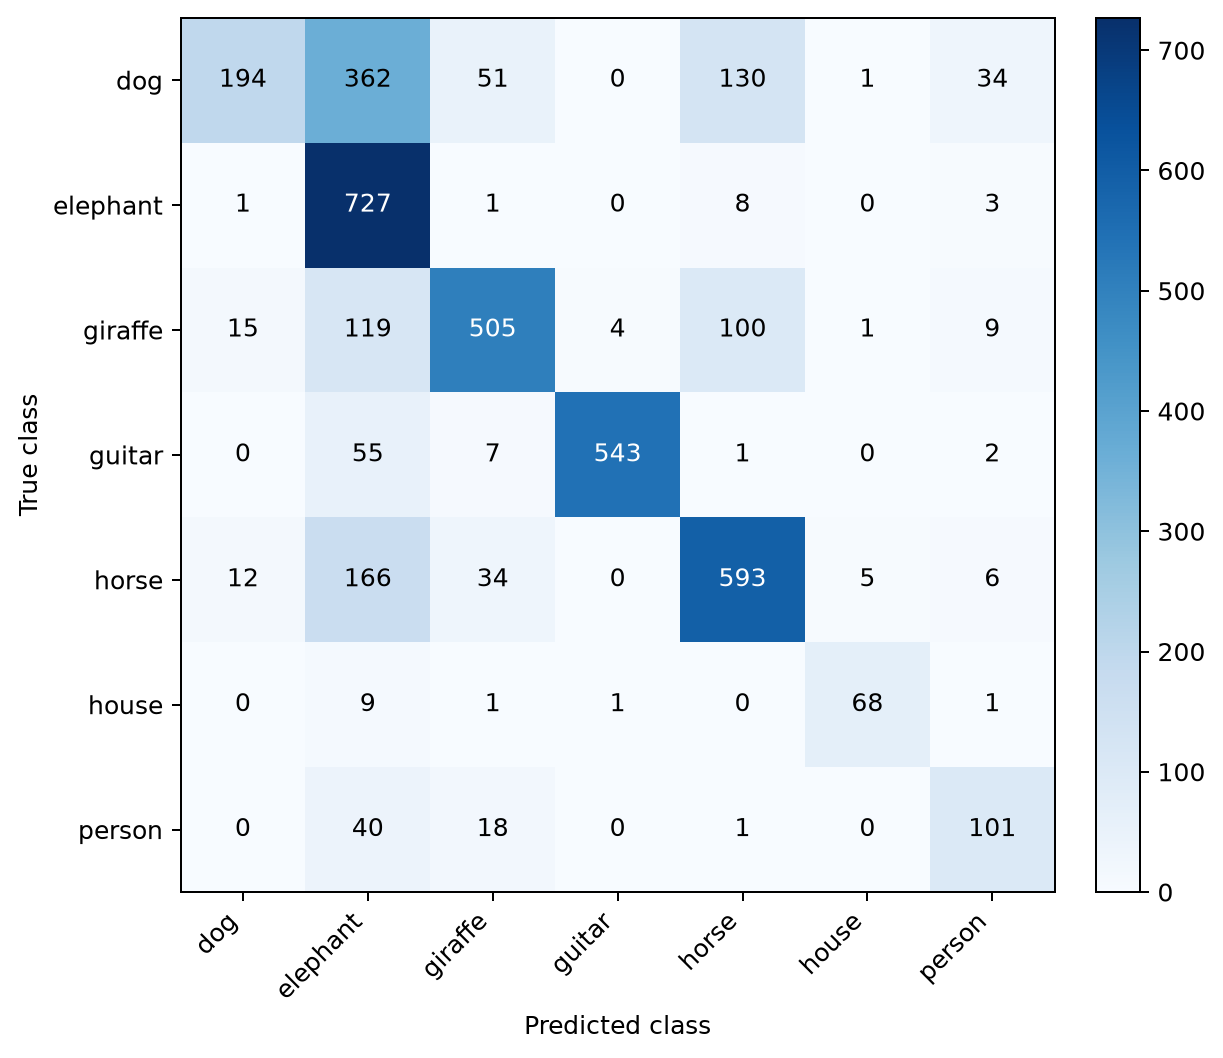
\includegraphics[width=\linewidth]{figures/pacs_confusion_sam.png}
\caption{SAM}\label{fig:pacsconfusion-sam}
\end{subfigure}
\caption{Target-domain confusion matrices for the DG methods. The shared ERM baseline appears in Fig.~\ref{fig:pacsconfusion-erm}. Rows show true classes, columns show predicted classes, and entries are image counts.}
\label{fig:pacsconfusion-dg}
\end{figure}

\end{document}
